% occuluded images
\section{Experiment}
We gathered a total of 16000 images for single and multi-lane highway as discussed in Chapter \ref{chap3}. From each of these images we randomly picked approximately 1200 pixels. This makes a total of 18,183,771 pixels. For each pixel we are storing their coordinates, the class it belongs to in a file and the image it is taken from as shown in \ref{lst:points_data}. The image from path information and the pixel coordinate are the input to our model and the class in shape of one-hot vector is the label. The model proposed in the previous chapter was executed with 80\% of the total pixels i.e 14,547,016. And the remaining 20\% pixels i.e 3,636,754 will be used for testing.

While implementing the model we faced some bugs or unwanted results as well. The process of locating and fixing defects or problems within a computer program or debugging is twice as hard as writing the program. Languages and frameworks usually provide documentation for debugging. In case of debugging neural networks in Tensorflow the challenge grows even more because of its working. Tensorboard is a effective tool provided by Google for debugging and visualizations.

We have visualized the conceptual graph of our proposed model's structure so we can easily explore and make sure that it matches our planned design. We can also view inputs, outputs and shapes through it. We can use name scopes to group together variables and operations as shown in the code \ref{lst:name_scope}:
\par
\begin{listing}
  \inputminted[frame=lines,framesep=2mm,baselinestretch=1.2,fontsize=\scriptsize,linenos]{python}{Chapter5/name_scope.py}
  \caption{Example usage of the name scope method}
  \label{lst:name_scope}
\end{listing}

\begin{figure}[H]
  \centering
  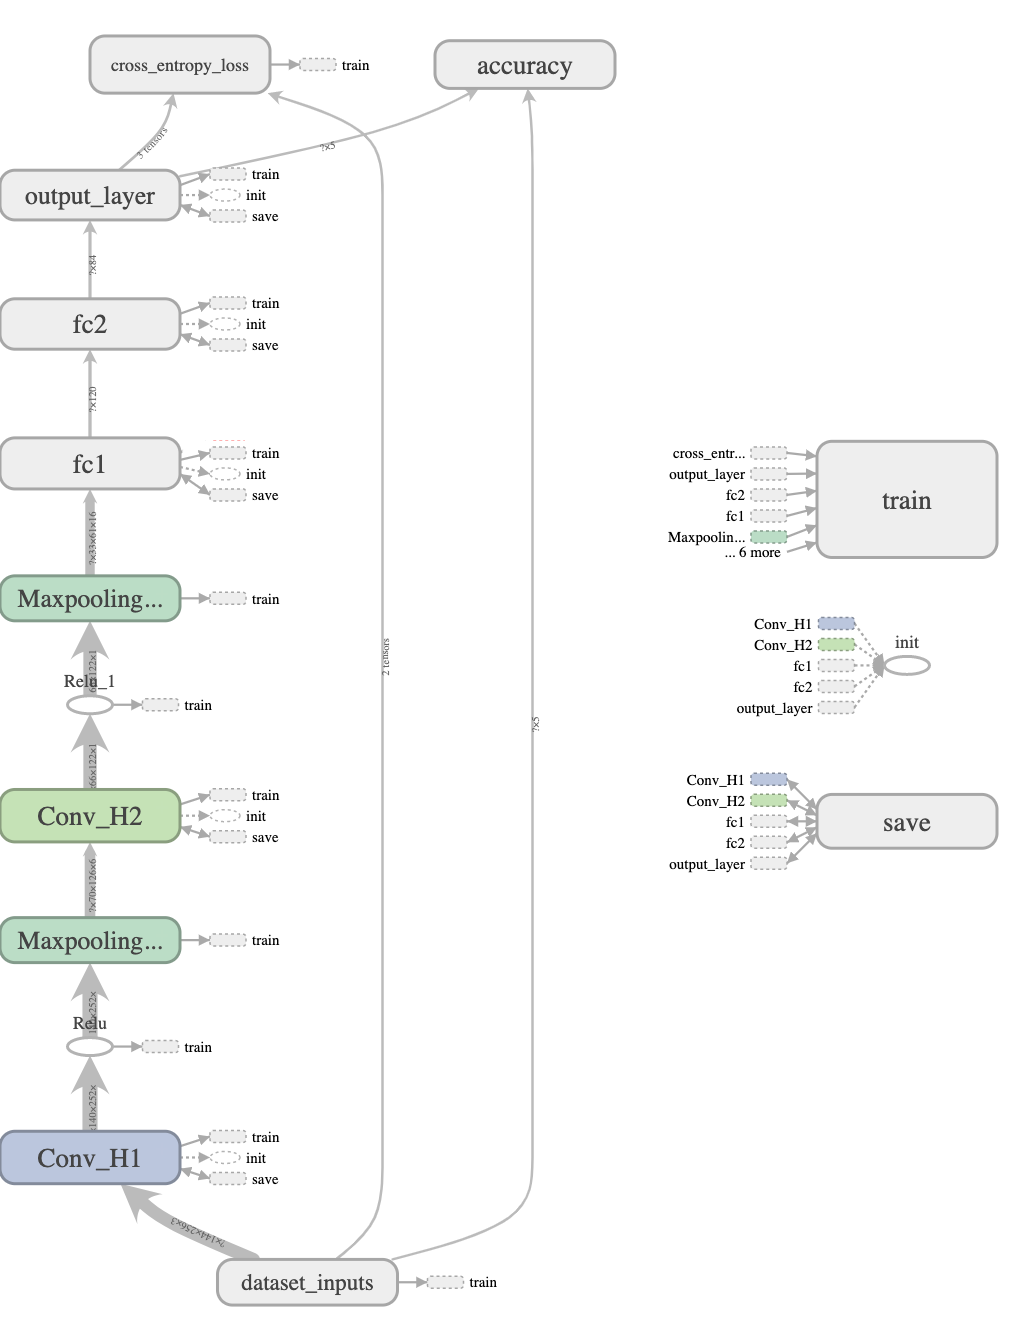
\includegraphics[scale=0.40]{images/Chapter5/graph.png}
  \caption{Tensorflow dataflow graph of our propesed model}
  \label{fig:graph}
\end{figure}

We can start the Tensorboard serve by run the following command in terminal:
\newline
\textbf{tensorboard --logdir=/tmp --port=3001}
\newline

Note, that we have added \textit{port} flag to the command. This is because our tensorboard server is running in the university's cluster and we have port-forwaded the port \textit{3001} so we can access it in my browser through http://localhost:3001/.

\section{Evaluation}
\subsection{Accuracy}
The Figure \ref{fig:accuracy} shows the accuracy of our model on training data. We trained our neural network with batch size of 128 for 10 epochs \ref{lst:log} with a sample size of 14,547,016 and got the final accuracy of 99\%. On running the same model on test data of 3,636,754 samples we get the accuracy of 98\%. Although, the accuracy of model is very good but it also indicates that either our data is very simple or we are overfitting.
\begin{figure}[H]
  \centering
  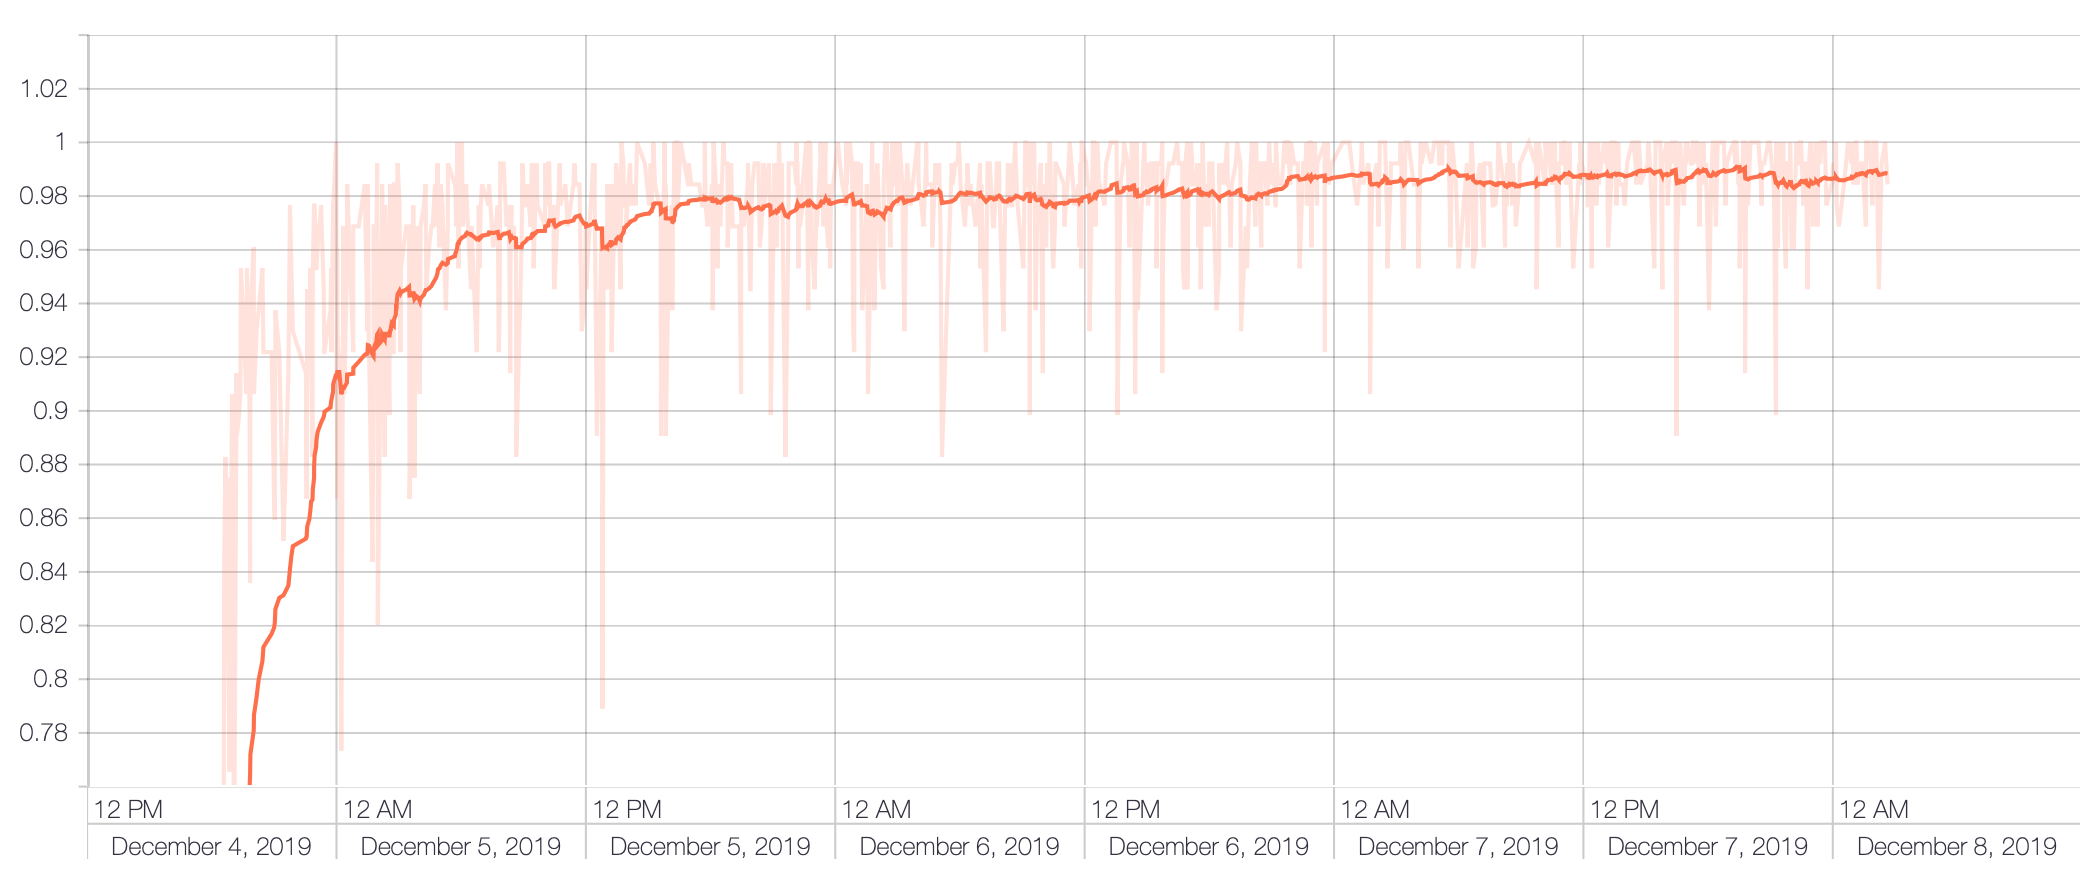
\includegraphics[scale=0.40]{images/Chapter5/accuracy.png}
  \caption{Accuracy of the trained }
  \label{fig:accuracy}
\end{figure}

\begin{listing}
  \inputminted[frame=lines,framesep=2mm,baselinestretch=1.2,fontsize=\scriptsize,linenos]{text}{Chapter5/epoch.txt}
  \caption{Training log}
  \label{lst:log}
\end{listing}

\subsection{Loss}
Cross Entropy Loss is usually used with multi-class classification problems. Cross Entropy Loss with Softmax function are used extensively as the output layer. Softmax function ensures normalization which means the sum of the components of the output vector is 1 and each one of them is positive and bounded. This function enhances the biggest values and suppresses the smallest values. We are using \textit{softmax\_cross\_entropy\_with\_logits\_v2} function of Tensorflow which gives softmax cross entropy between labels and logits. The loss value graph is shown in Figure \ref{fig:loss}. The lowest the loss value is, the better a model is trained. After 10 Epochs we got a loss value of 0.025985, which is agood sign.
\begin{figure}[H]
  \centering
  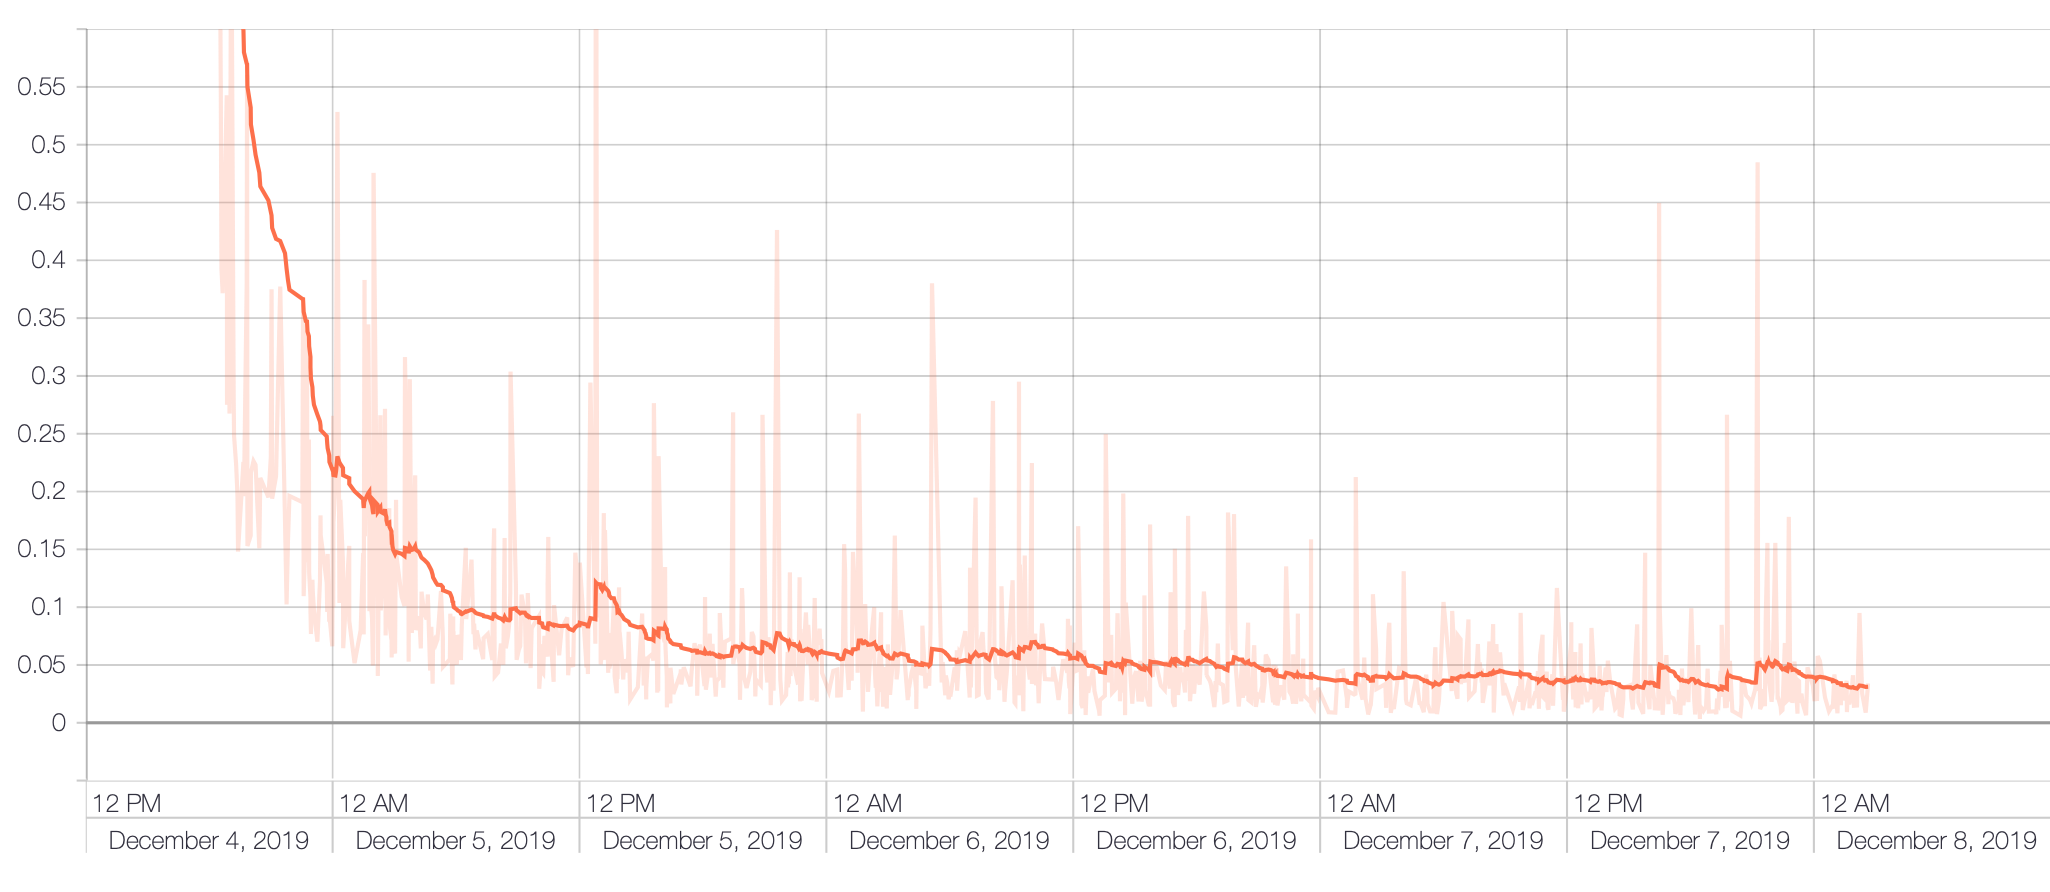
\includegraphics[scale=0.40]{images/Chapter5/loss.png}
  \caption{Softmax cross-entropy loss}
  \label{fig:loss}
\end{figure}


\subsection{Visualization}
Visualization is a powerful tool to communicate ideas, tell a story or show results in the form of graphs, charts, or maps. It is also helpful in finding patterns. Although, our model accuracy is very good, we wrote a script \ref{lst:visualize} to visualize our predictions in order show the results in human understandable form. First of all we are generating a grid of point coordinates in the area we are most interested in. ThenNote that each point is a separate prediction plotted on the respective image. As we discussed in previous chapter, our model takes in an image as input with point coordinates to predict. So we put the point coordinates in the last pixel of the image. Then we are restoring the trained model which was saved during the training process. Getting the output of the trained model tells us, to which lane or outside of lane does the point coordinate belongs to. We color coded the predicted points as shown in Table \ref{color_code_visualization}. Each predicted point is plotted at the respective coordinate over the image. With the help of background image we can identify wheater the predicted points are correctly classified.
\begin{listing}
  \inputminted[frame=lines,framesep=2mm,baselinestretch=1.2,fontsize=\scriptsize,linenos]{python}{Chapter5/visualize.py}
  \caption{Script to visualize predicted points on the image}
  \label{lst:visualize}
\end{listing}
\begin{table}[H]
  \centering
  \begin{tabular}{ |c|c| }
    \hline
    \textbf{Predicted Class} & \textbf{RGB Color Code} \\
    \hline
    Outside & rgb(   0,   0,   0) \thiscolor{black}\\
    \hline
    Lane-1 & rgb(   0,   0, 255) \thiscolor{blue}\\
    \hline
    Lane-2 & rgb(   0, 255,   0) \thiscolor{green}\\
    \hline
    Lane-3 & rgb( 255,   0,   0) \thiscolor{red}\\
    \hline
    Lane-4 & rgb( 255, 255, 255) \thiscolor{white}\\
    \hline
  \end{tabular}
\caption{Predicted points color coded for visualization}
\label{color_code_visualization}
\end{table}

\par
This means that if the given point is predicted as \textit{lane1} (the right-most lane) then color of the point will be blue and so on. This will help us understand whether our model has just memorized the road shape or giving results based on the visual features. It will also help us find patterns when predictions are incorrect.
% This will help us understand whether our model is predicting the points 
\par
The Figures \ref{fig:good-straight-1}, \ref{fig:good-straight-2}, \ref{fig:good-straight-3} and \ref{fig:good-straight-4} shows that results on straight roads were very good.

\begin{figure}[H]
  \centering
  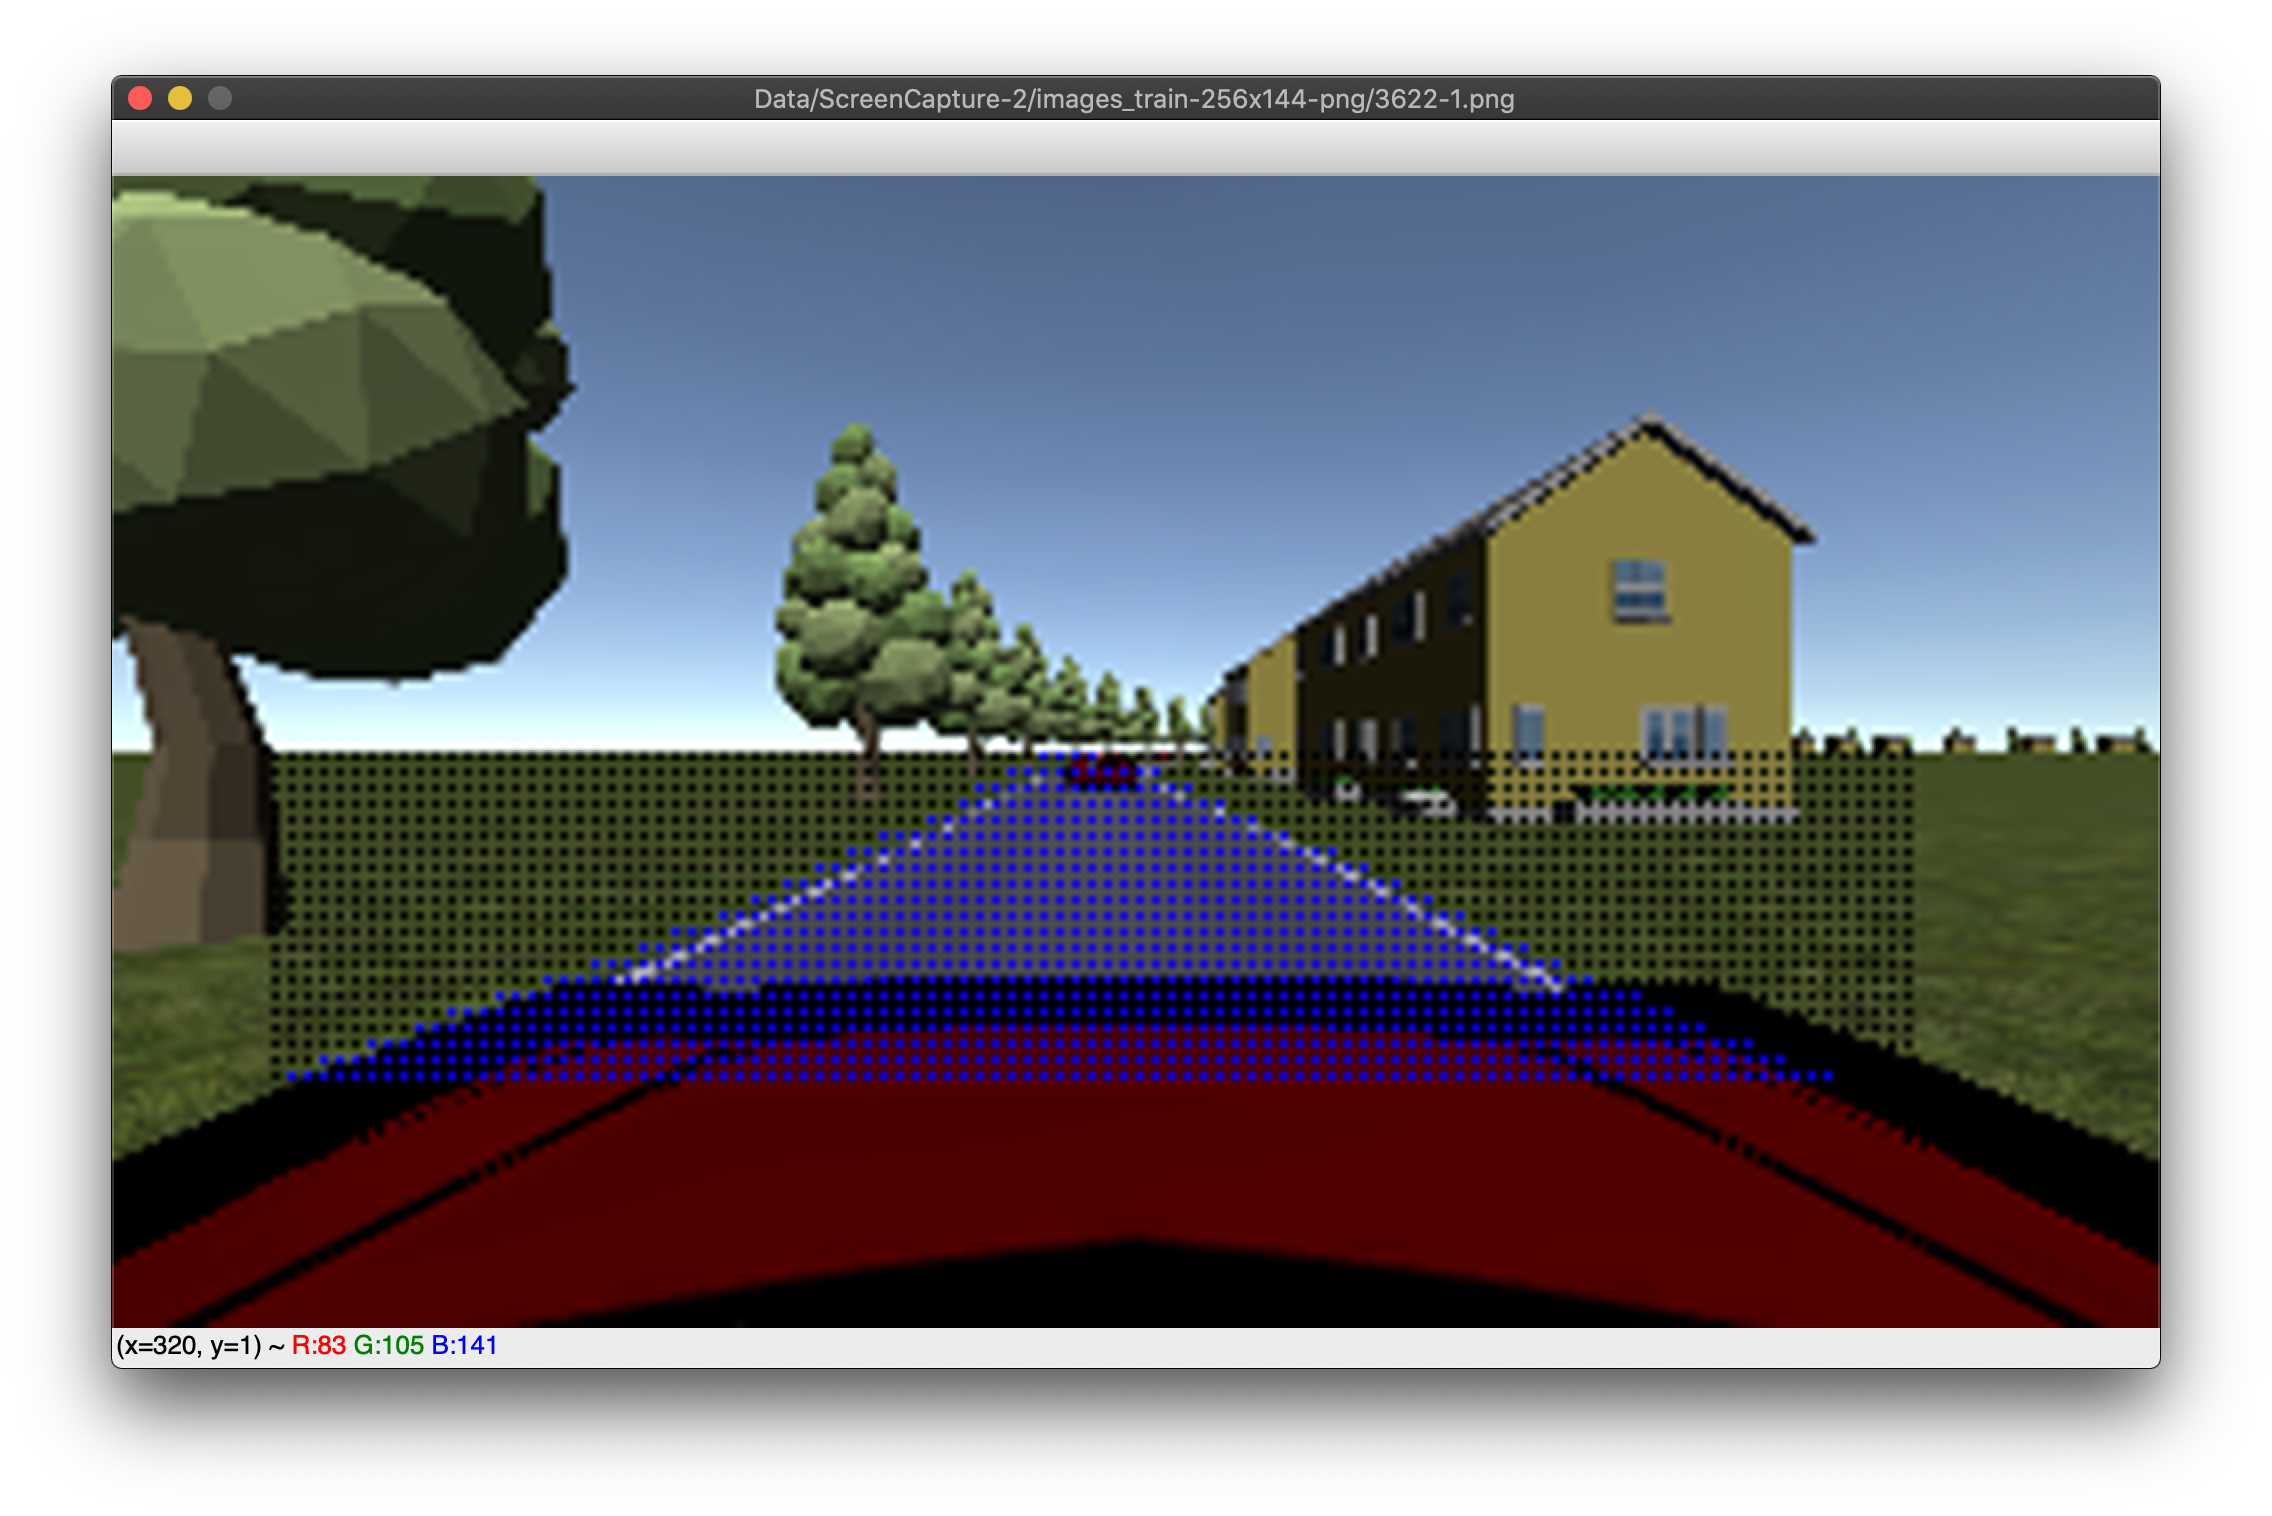
\includegraphics[scale=0.31]{images/Chapter5/lane1-straight-green.png}
  \caption{Good results on straight 1-lane highway}
  \label{fig:good-straight-1}
\end{figure}
\begin{figure}[H]
  \centering
  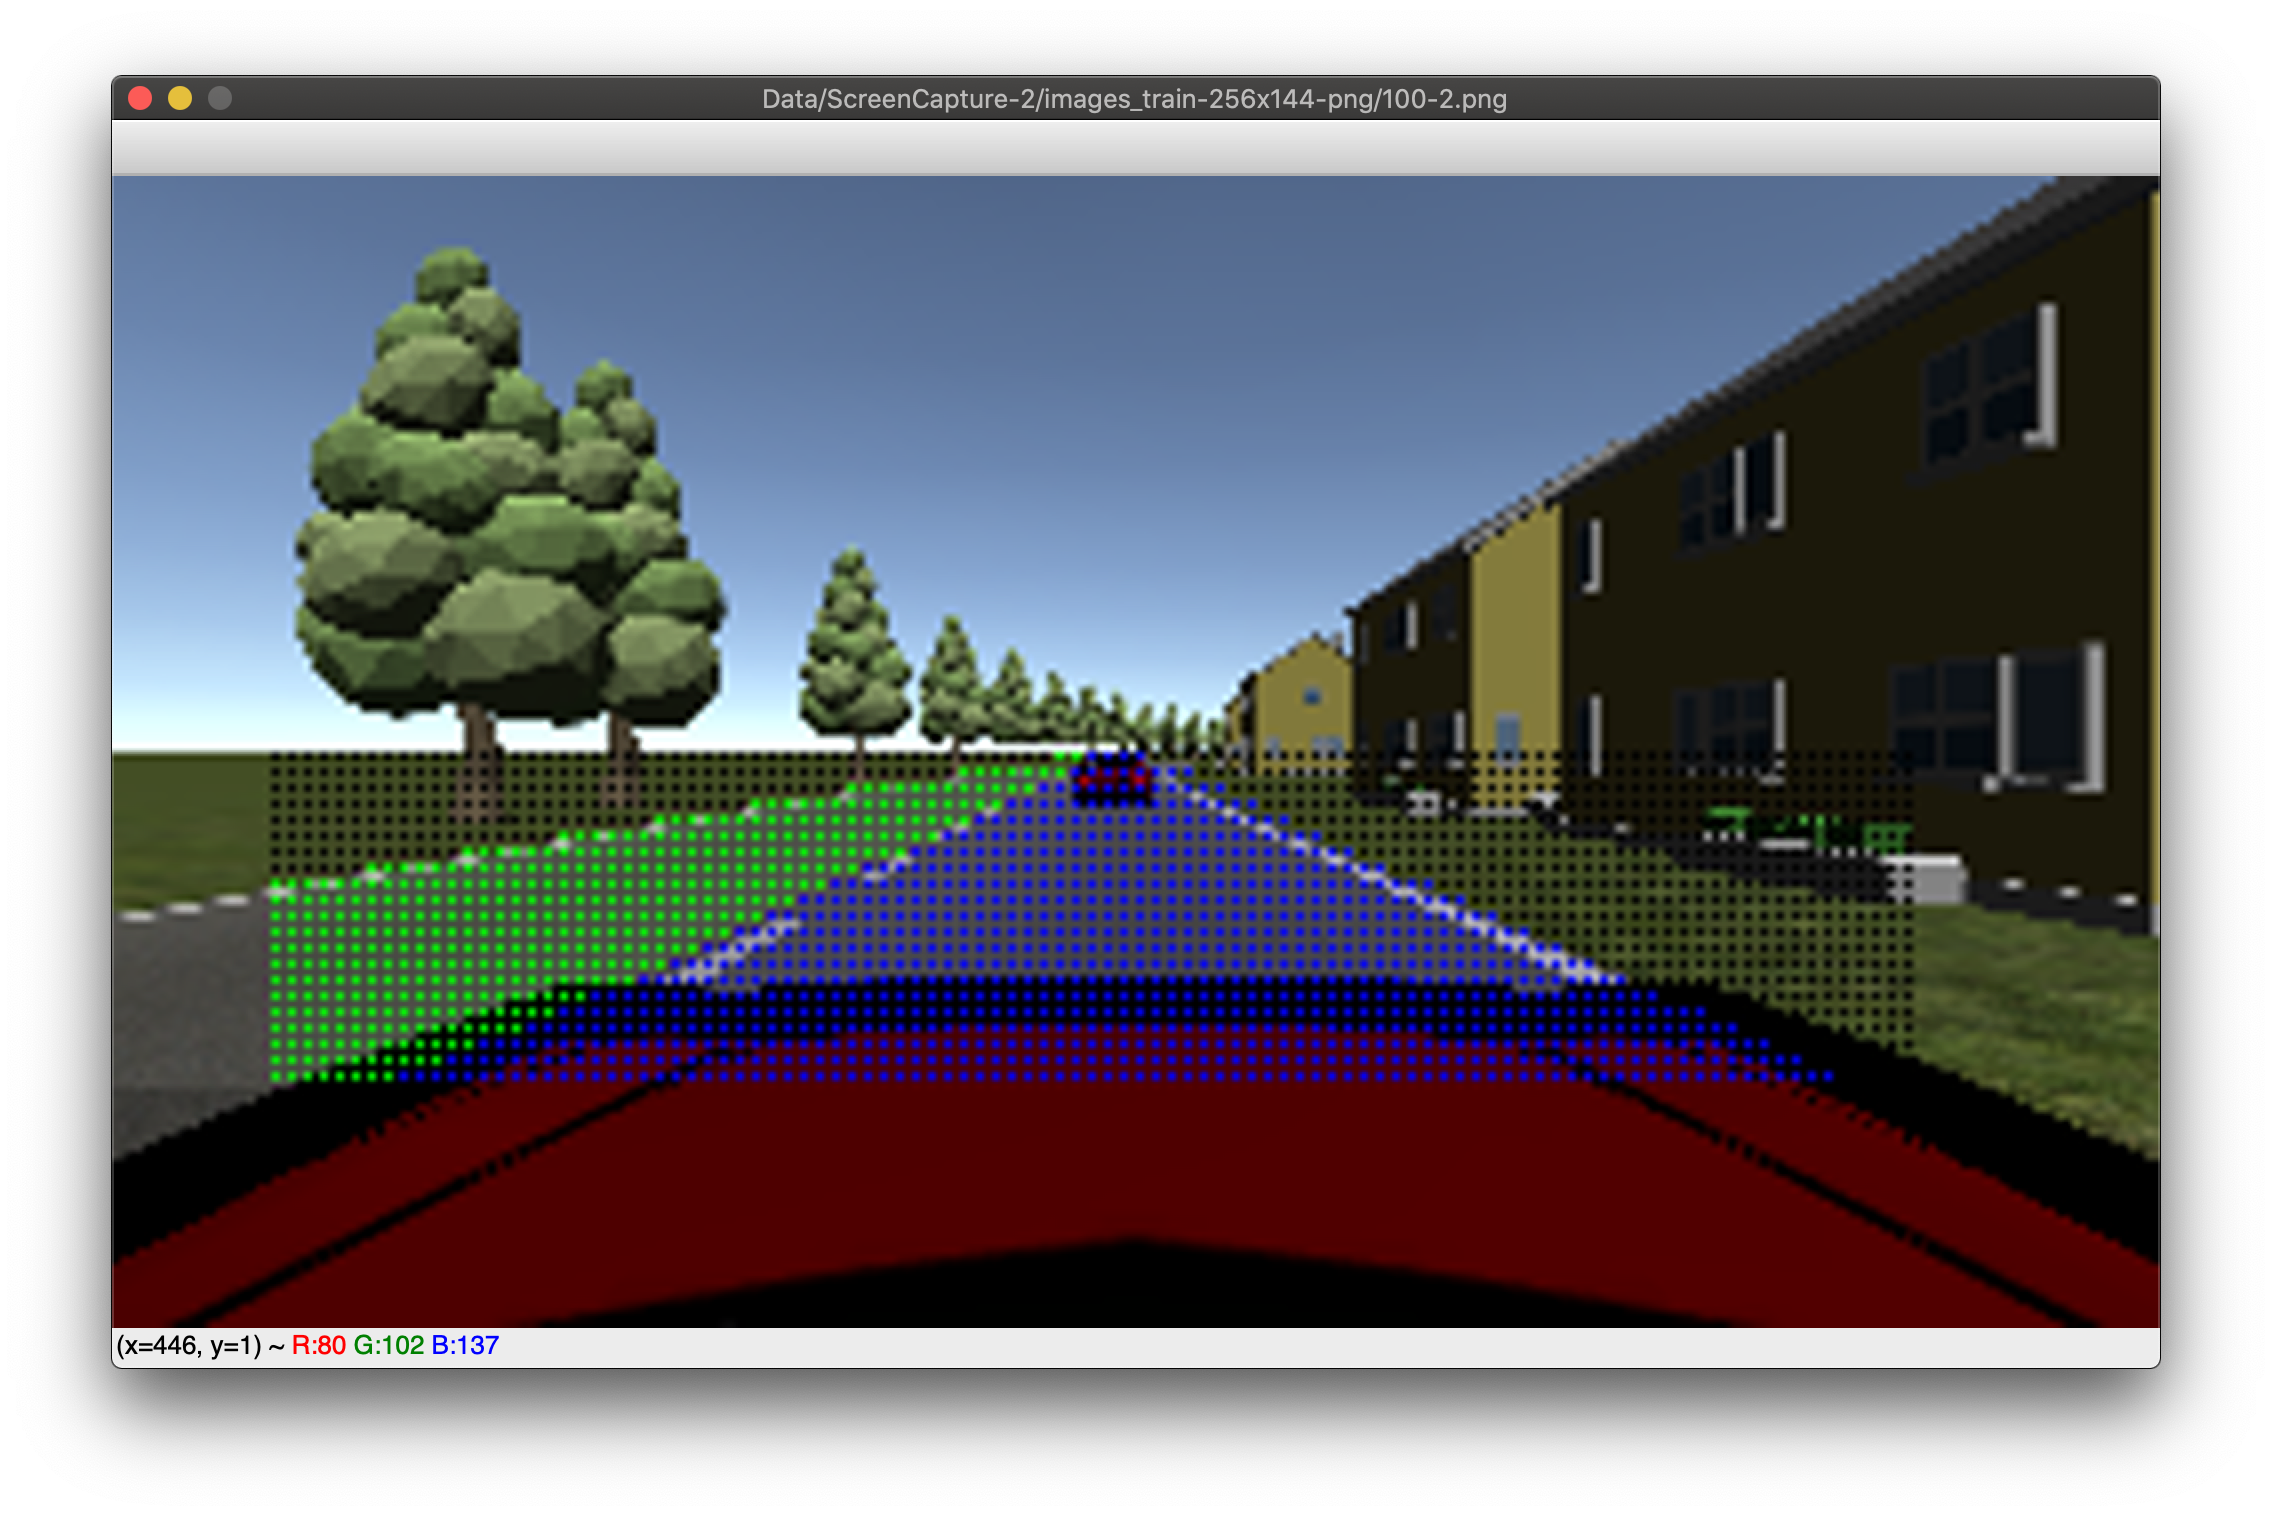
\includegraphics[scale=0.31]{images/Chapter5/lane2-straight-green.png}
  \caption{Good results on straight 2-lane highway}
  \label{fig:good-straight-2}
\end{figure}
\begin{figure}[H]
  \centering
  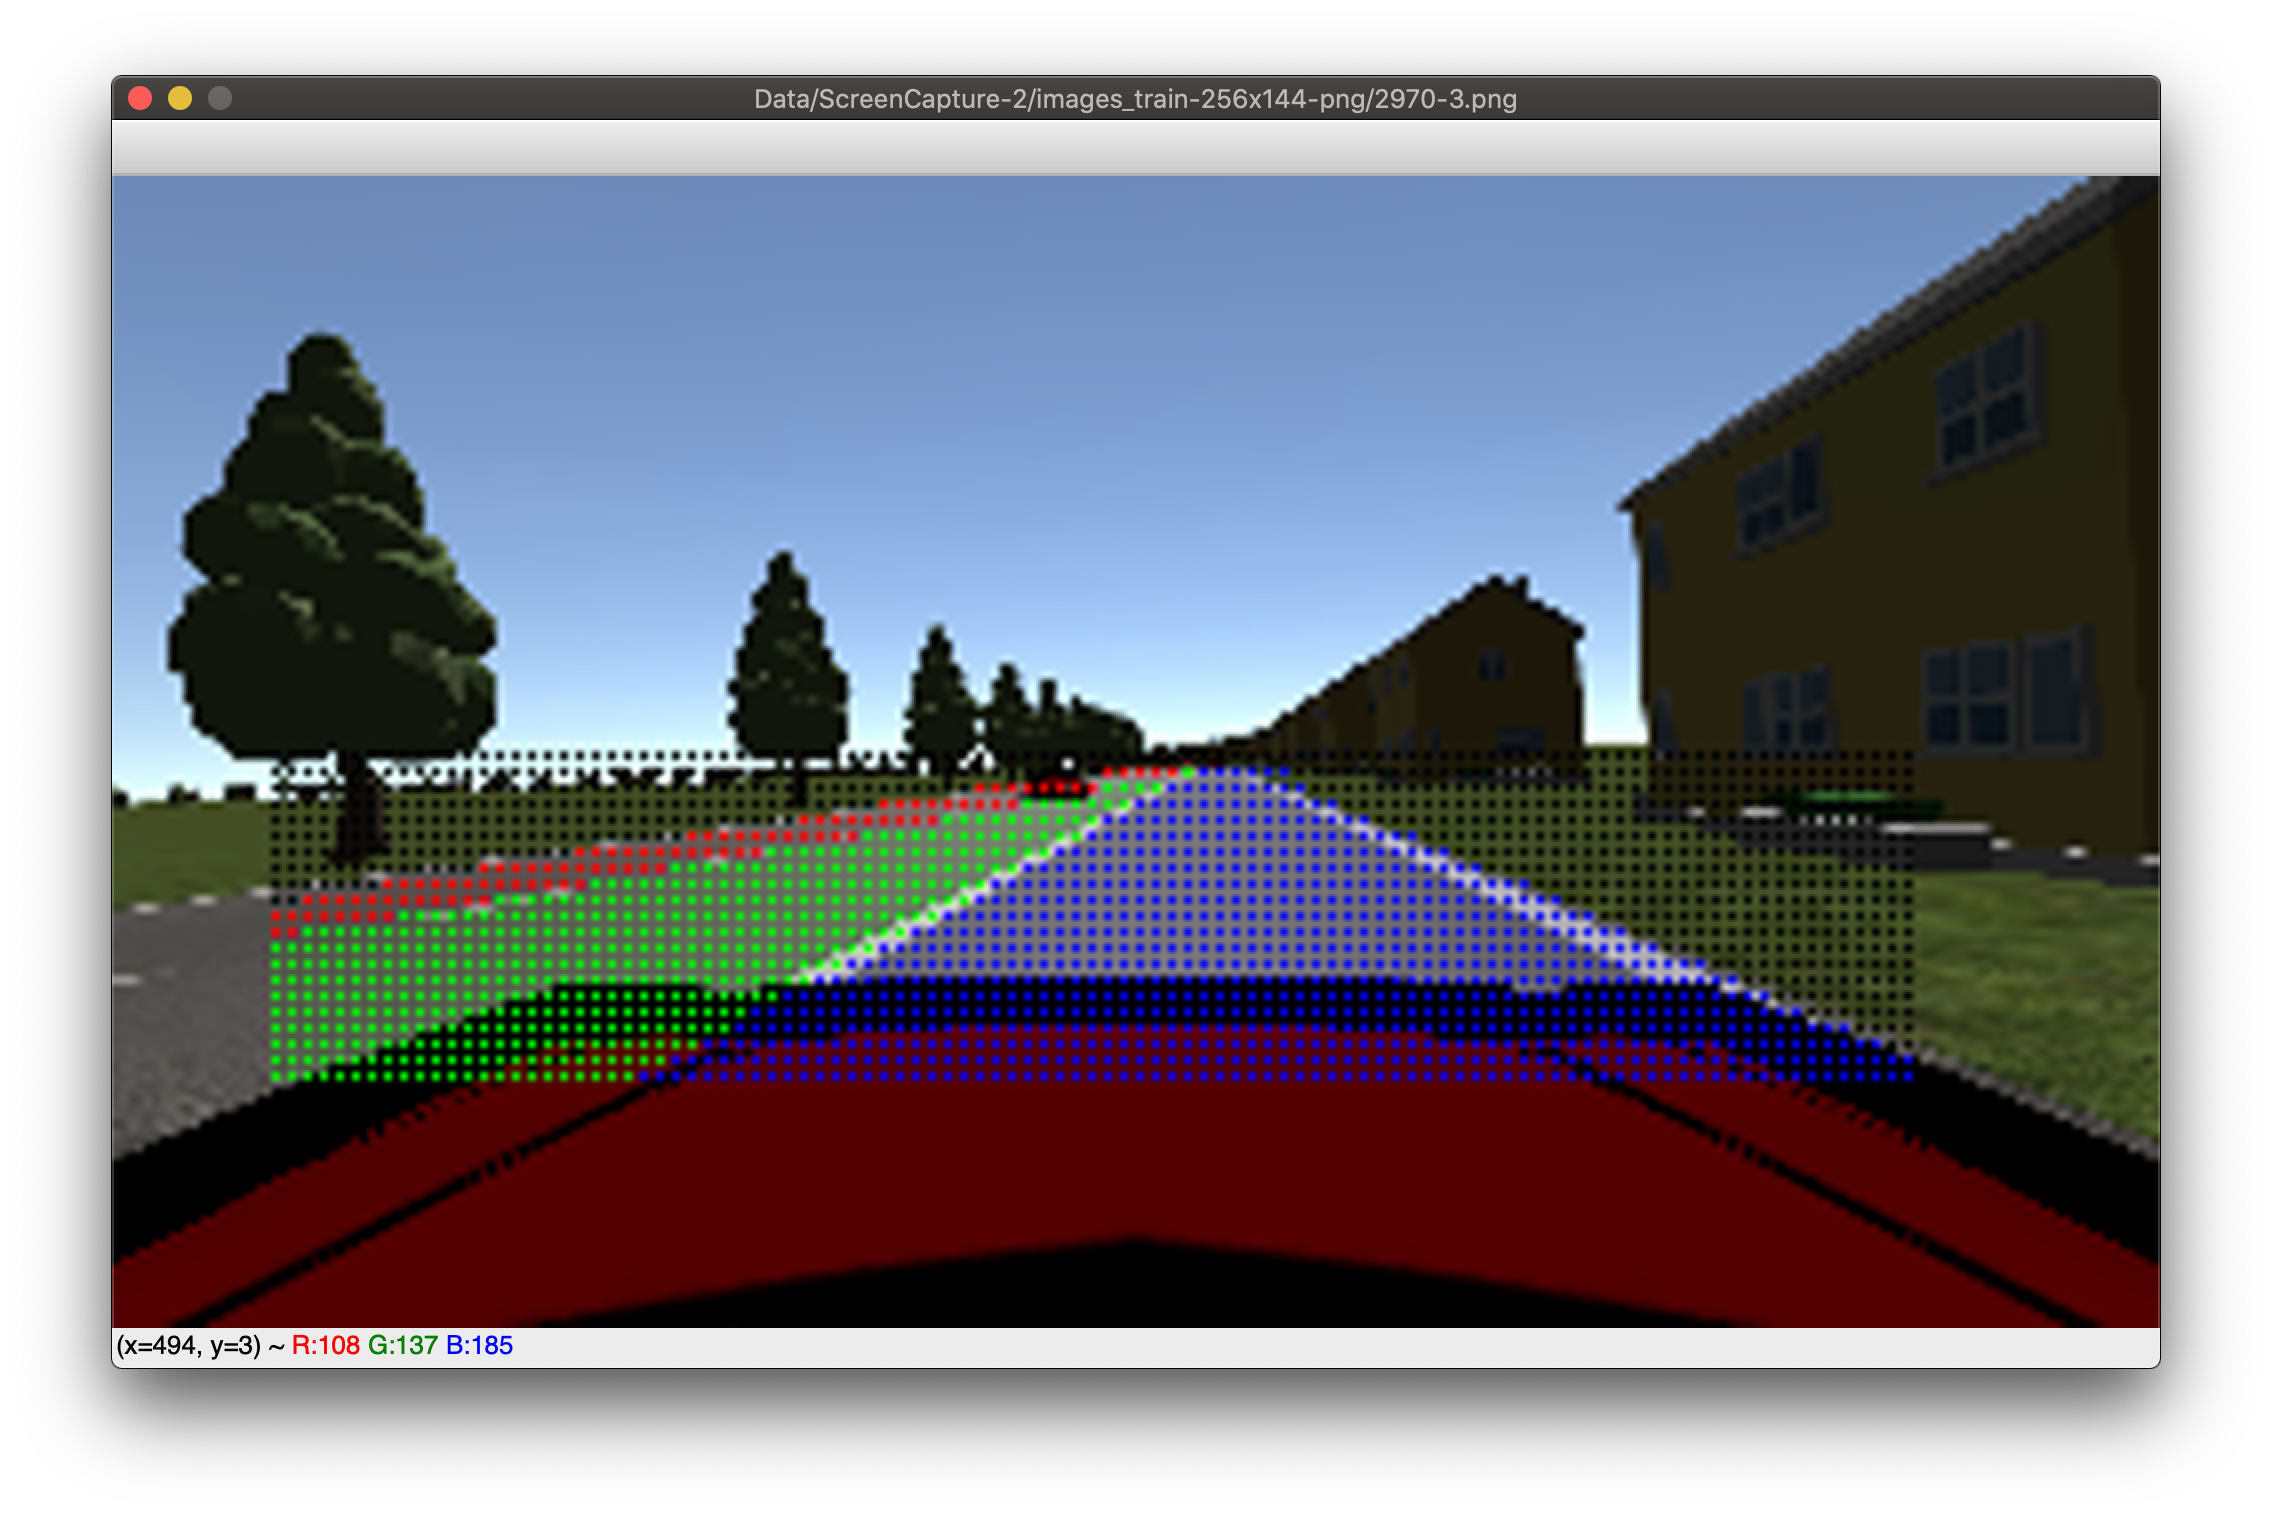
\includegraphics[scale=0.31]{images/Chapter5/lane3-straight-green.png}
  \caption{Good results on straight 3-lane highway}
  \label{fig:good-straight-3}
\end{figure}
\begin{figure}[H]
  \centering
  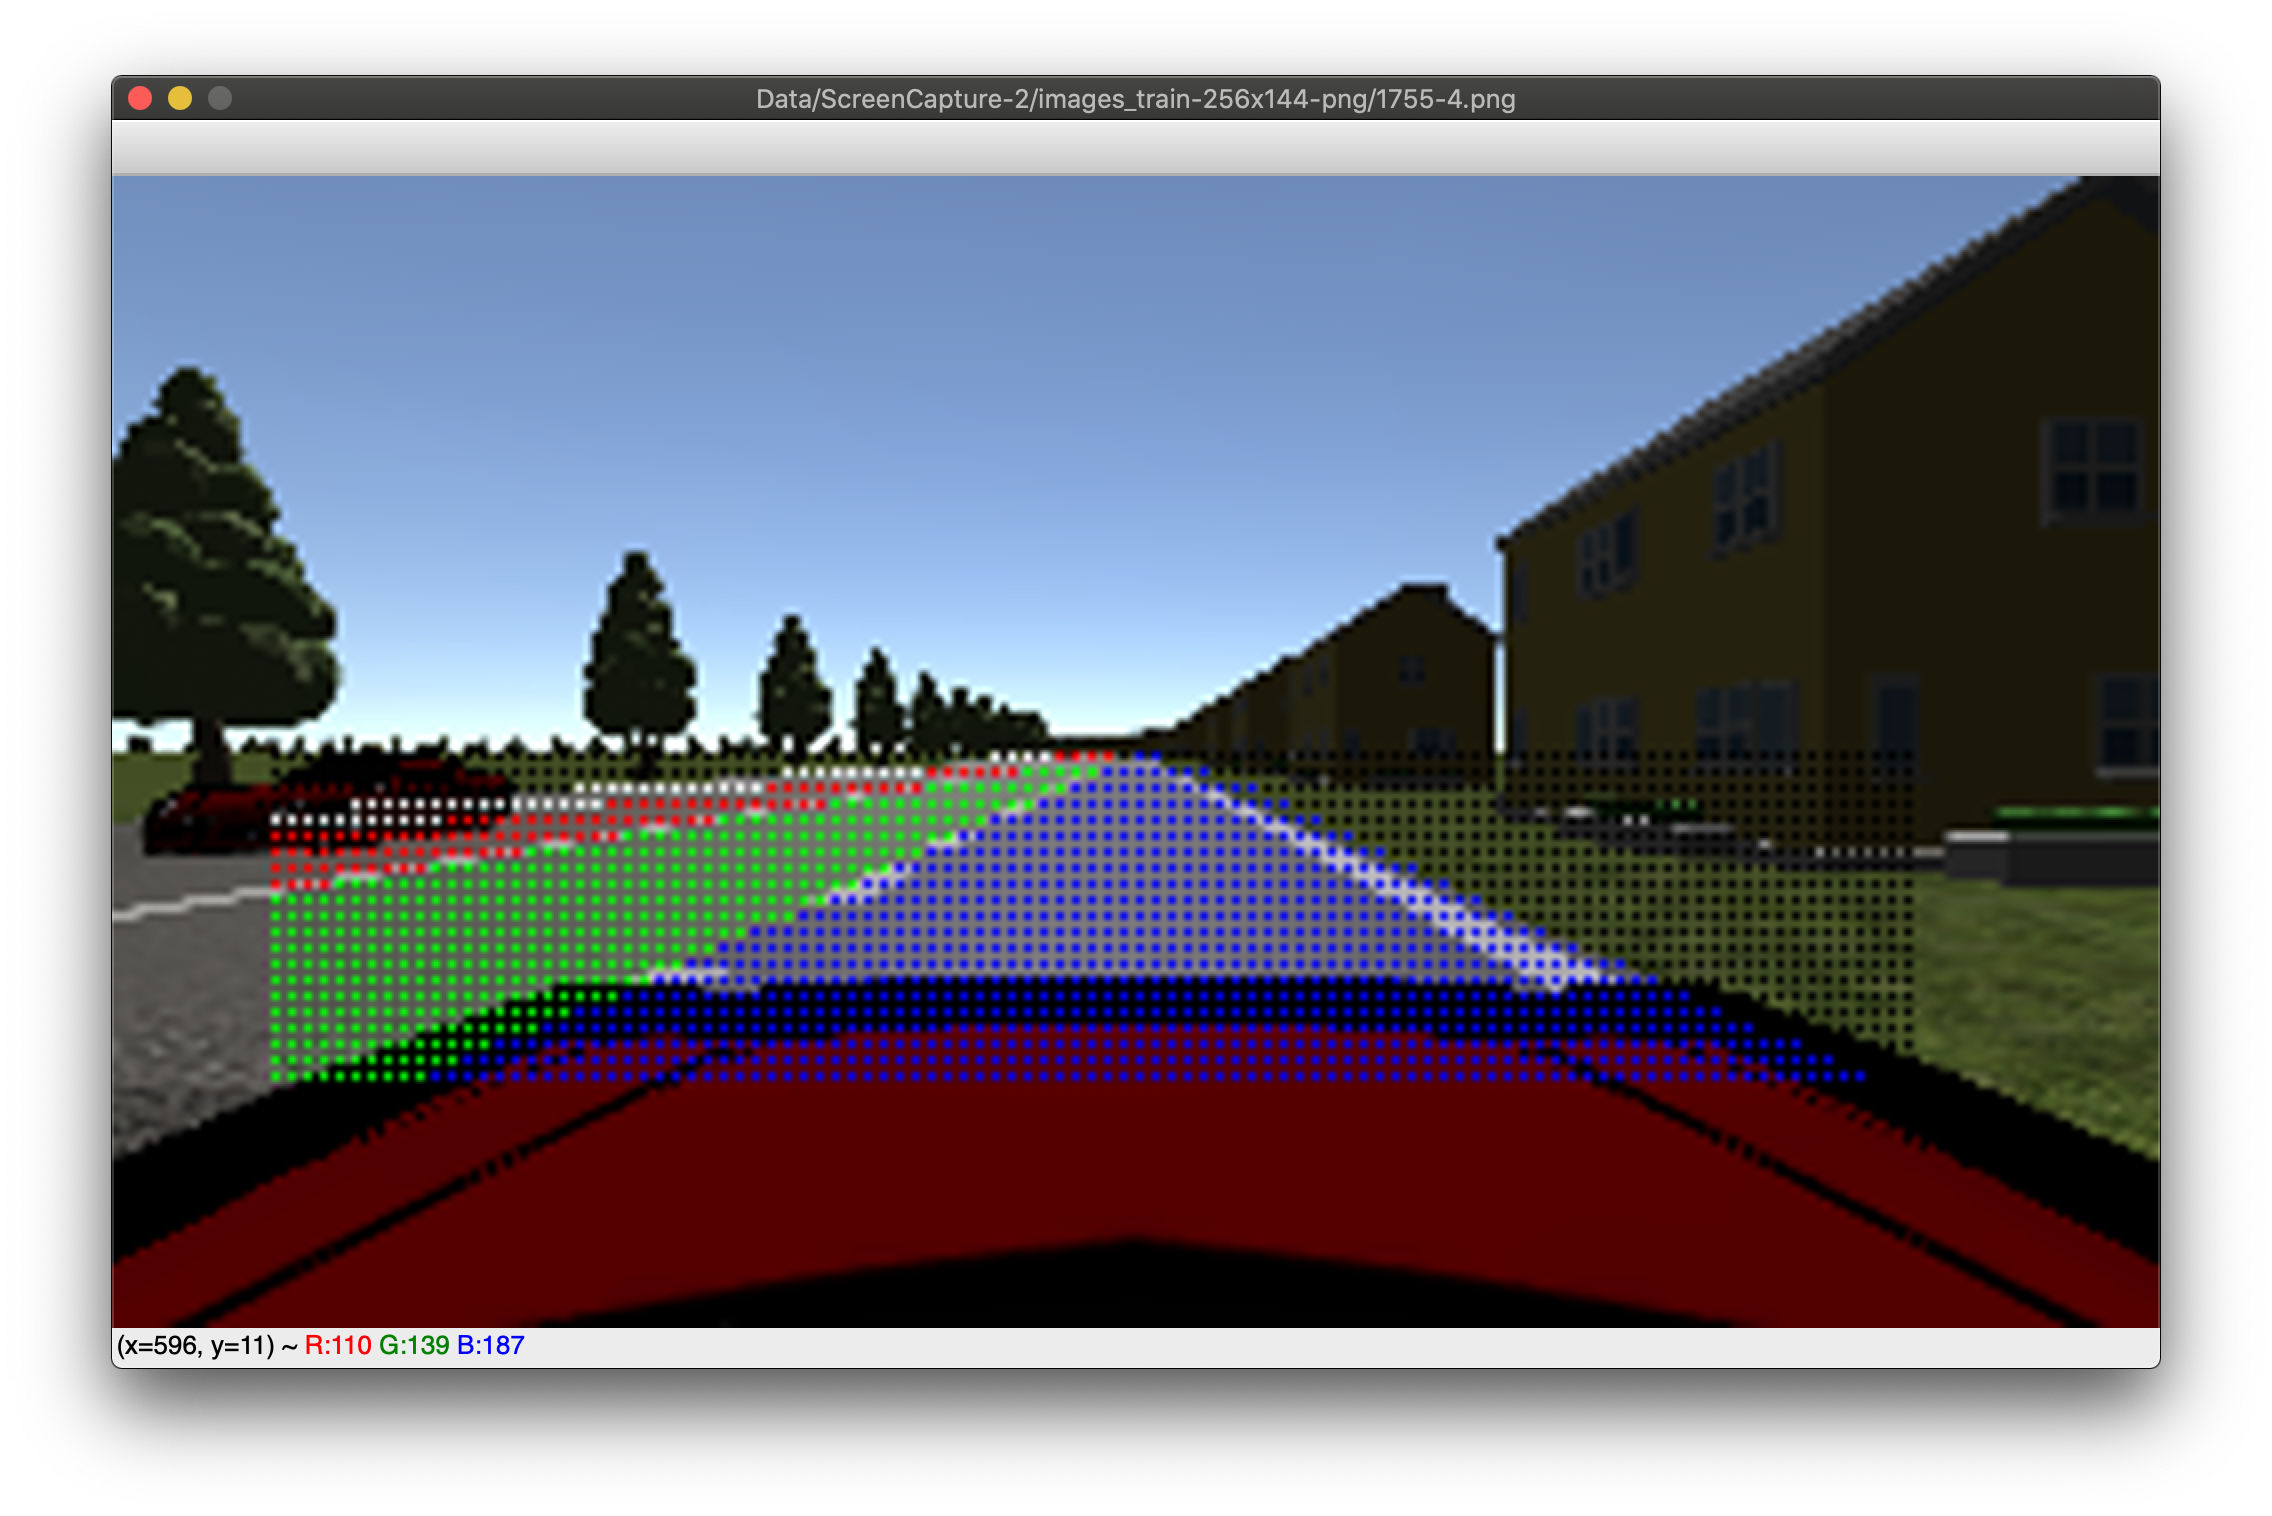
\includegraphics[scale=0.31]{images/Chapter5/lane4-straight-green.png}
  \caption{Good results on straight 4-lane highway}
  \label{fig:good-straight-4}
\end{figure}

\par
Not only the straight roads, the Figures \ref{fig:good-curve-1}, \ref{fig:good-curve-2}, \ref{fig:good-curve-3} and \ref{fig:good-curve-4} shows that of the results were also good in most of the on curved roads as well. Although, we do not have images with sharp turns but we can see the curve in predicted points which shows that our model has not simply memorized the road shapes.

\begin{figure}[H]
  \centering
  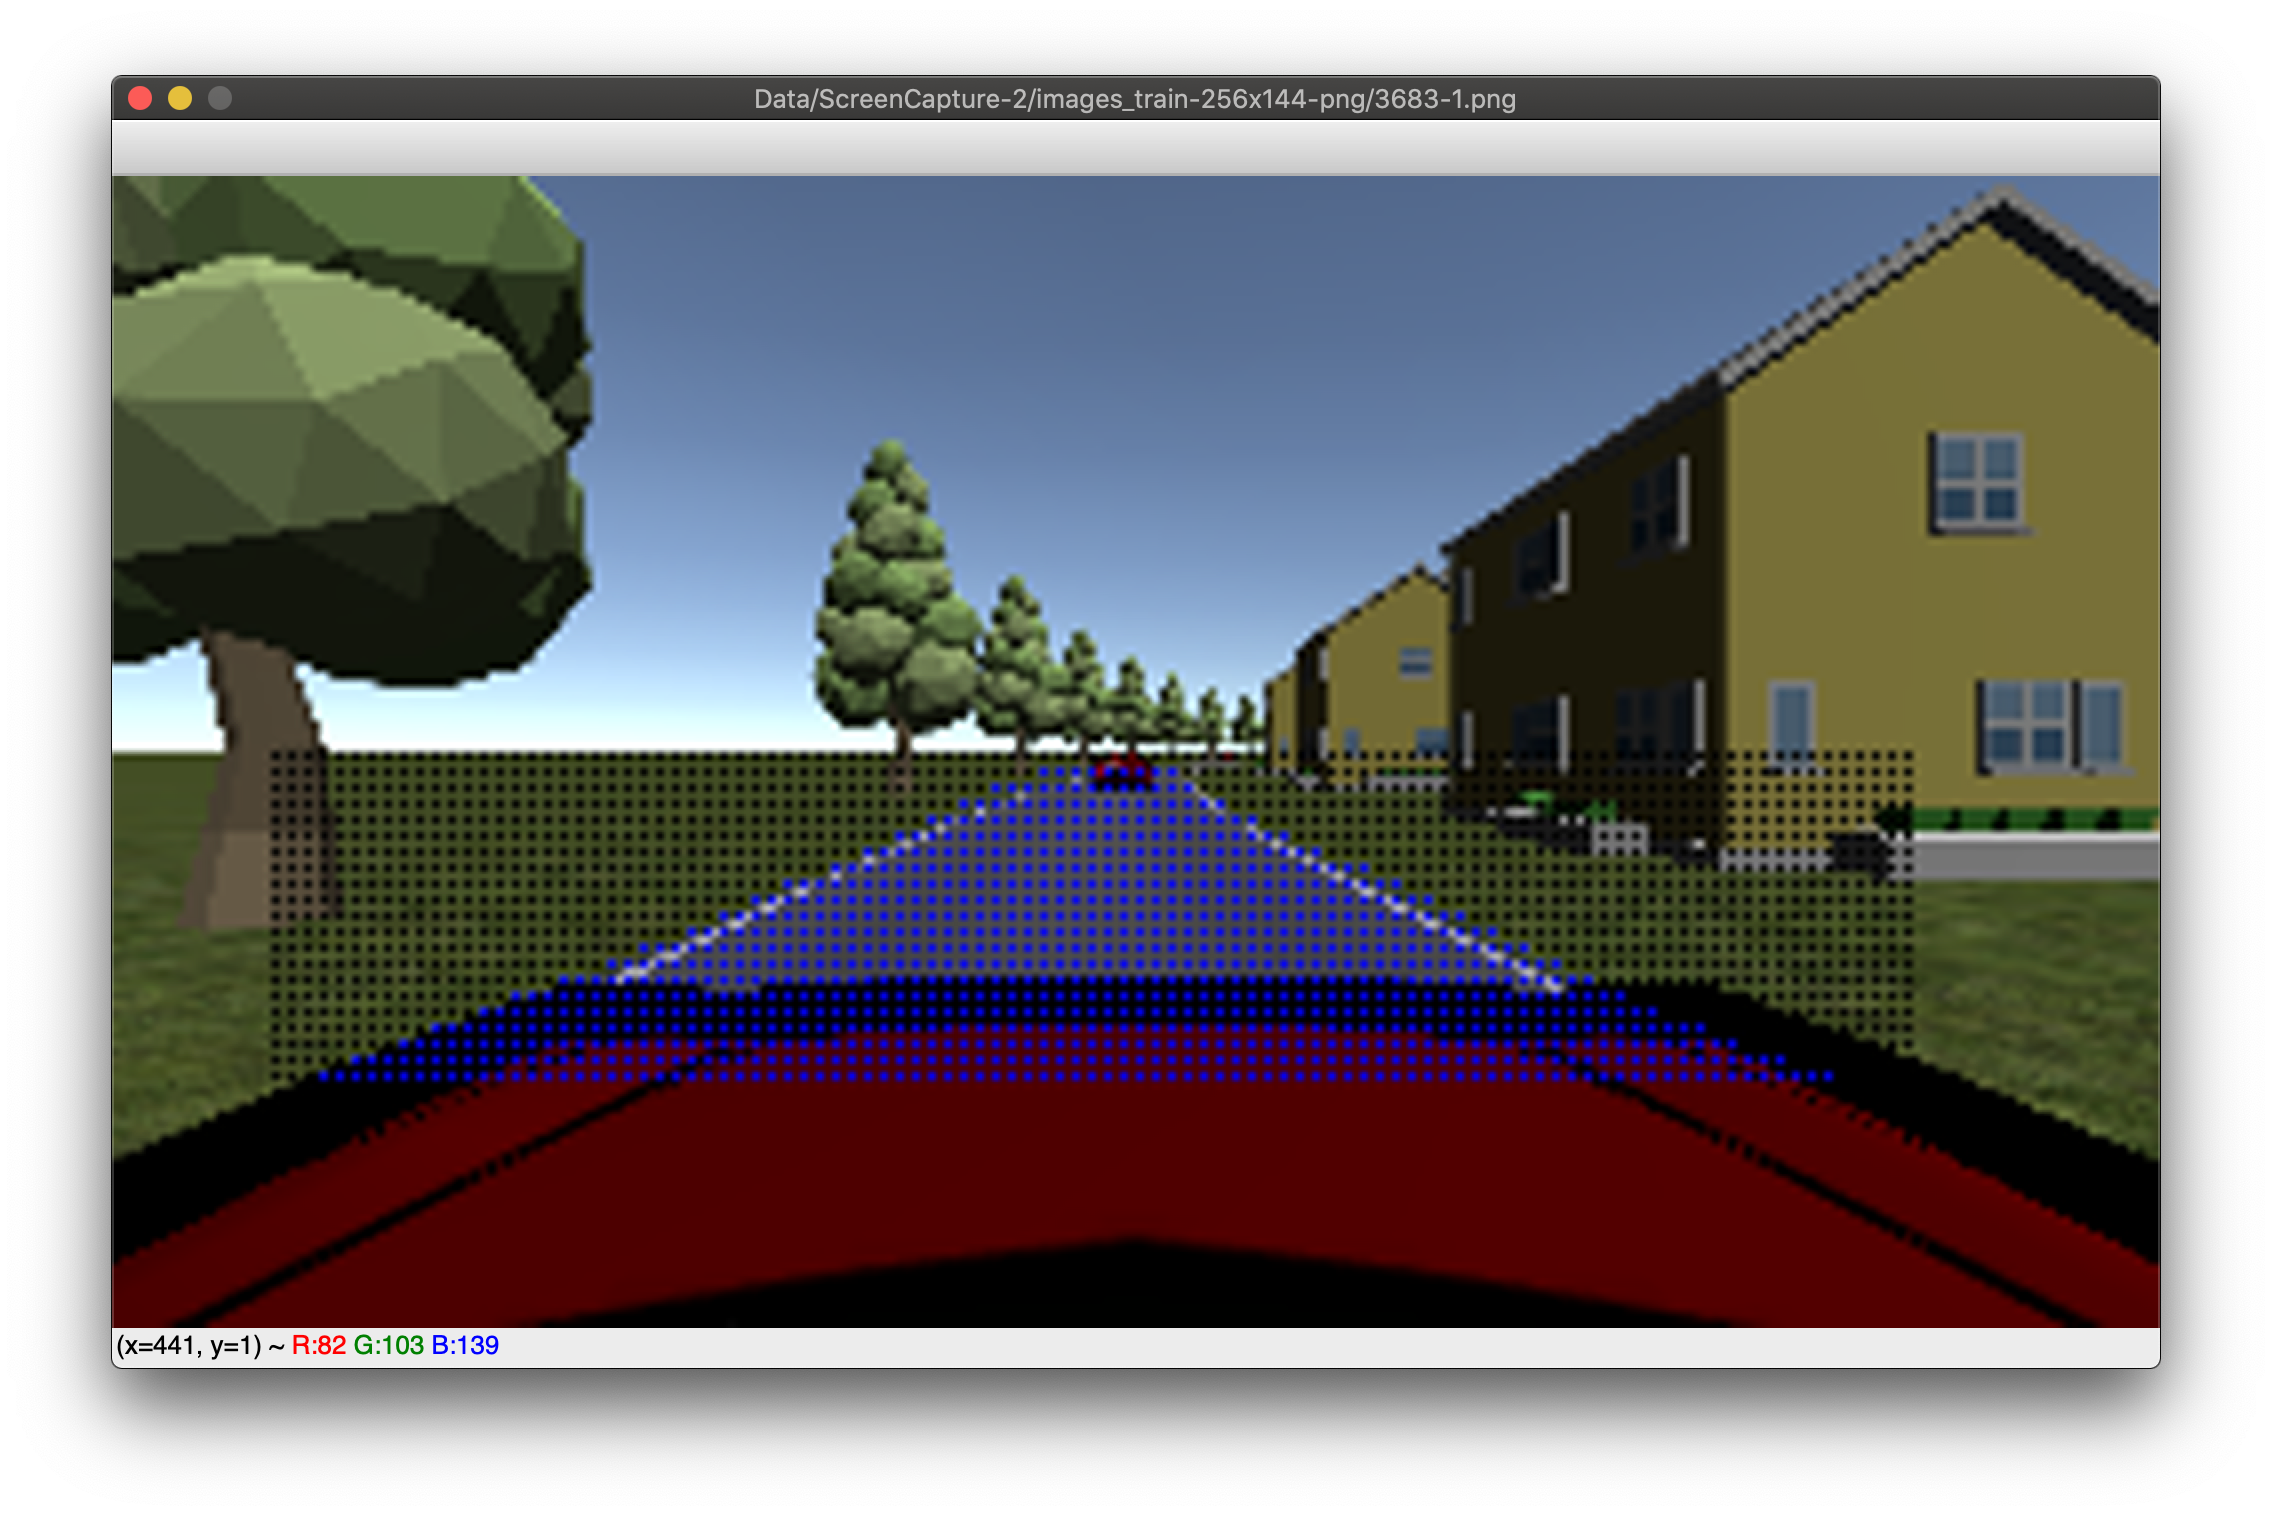
\includegraphics[scale=0.31]{images/Chapter5/lane1-curve-green.png}
  \caption{Good results on curved 1-lane highway}
  \label{fig:good-curve-1}
\end{figure}
\begin{figure}[H]
  \centering
  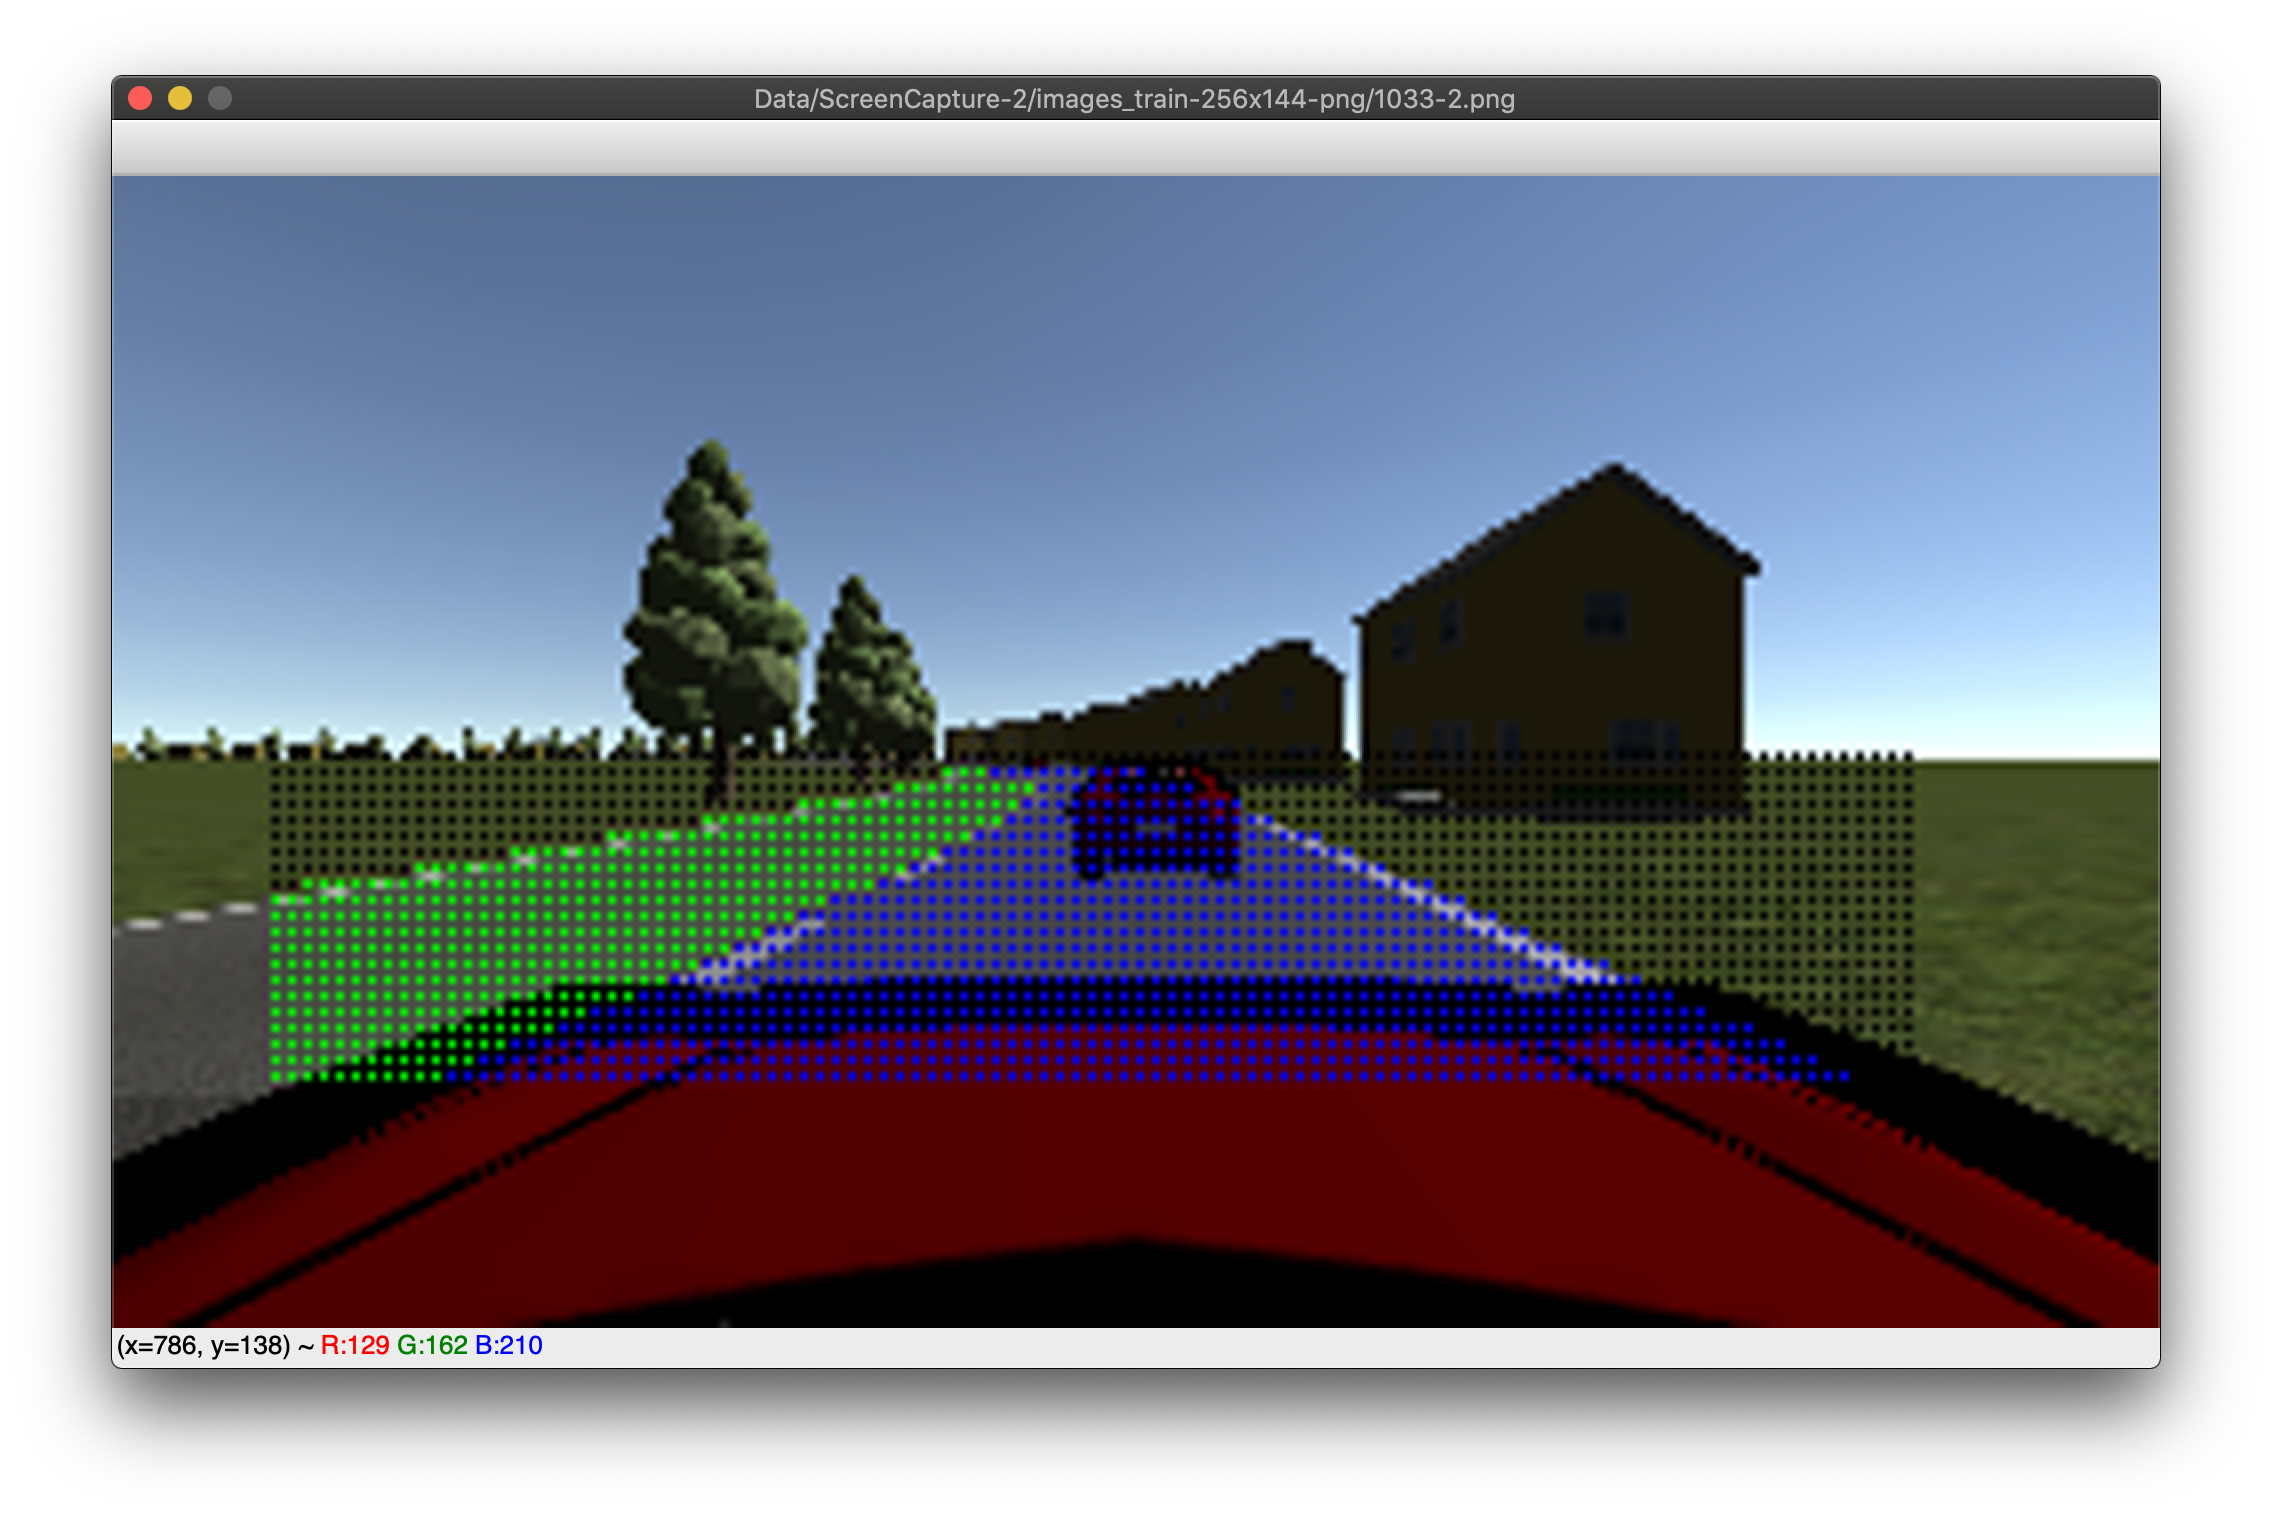
\includegraphics[scale=0.31]{images/Chapter5/lane2-curve-green.png}
  \caption{Good results on curved 2-lane highway}
  \label{fig:good-curve-2}
\end{figure}
\begin{figure}[H]
  \centering
  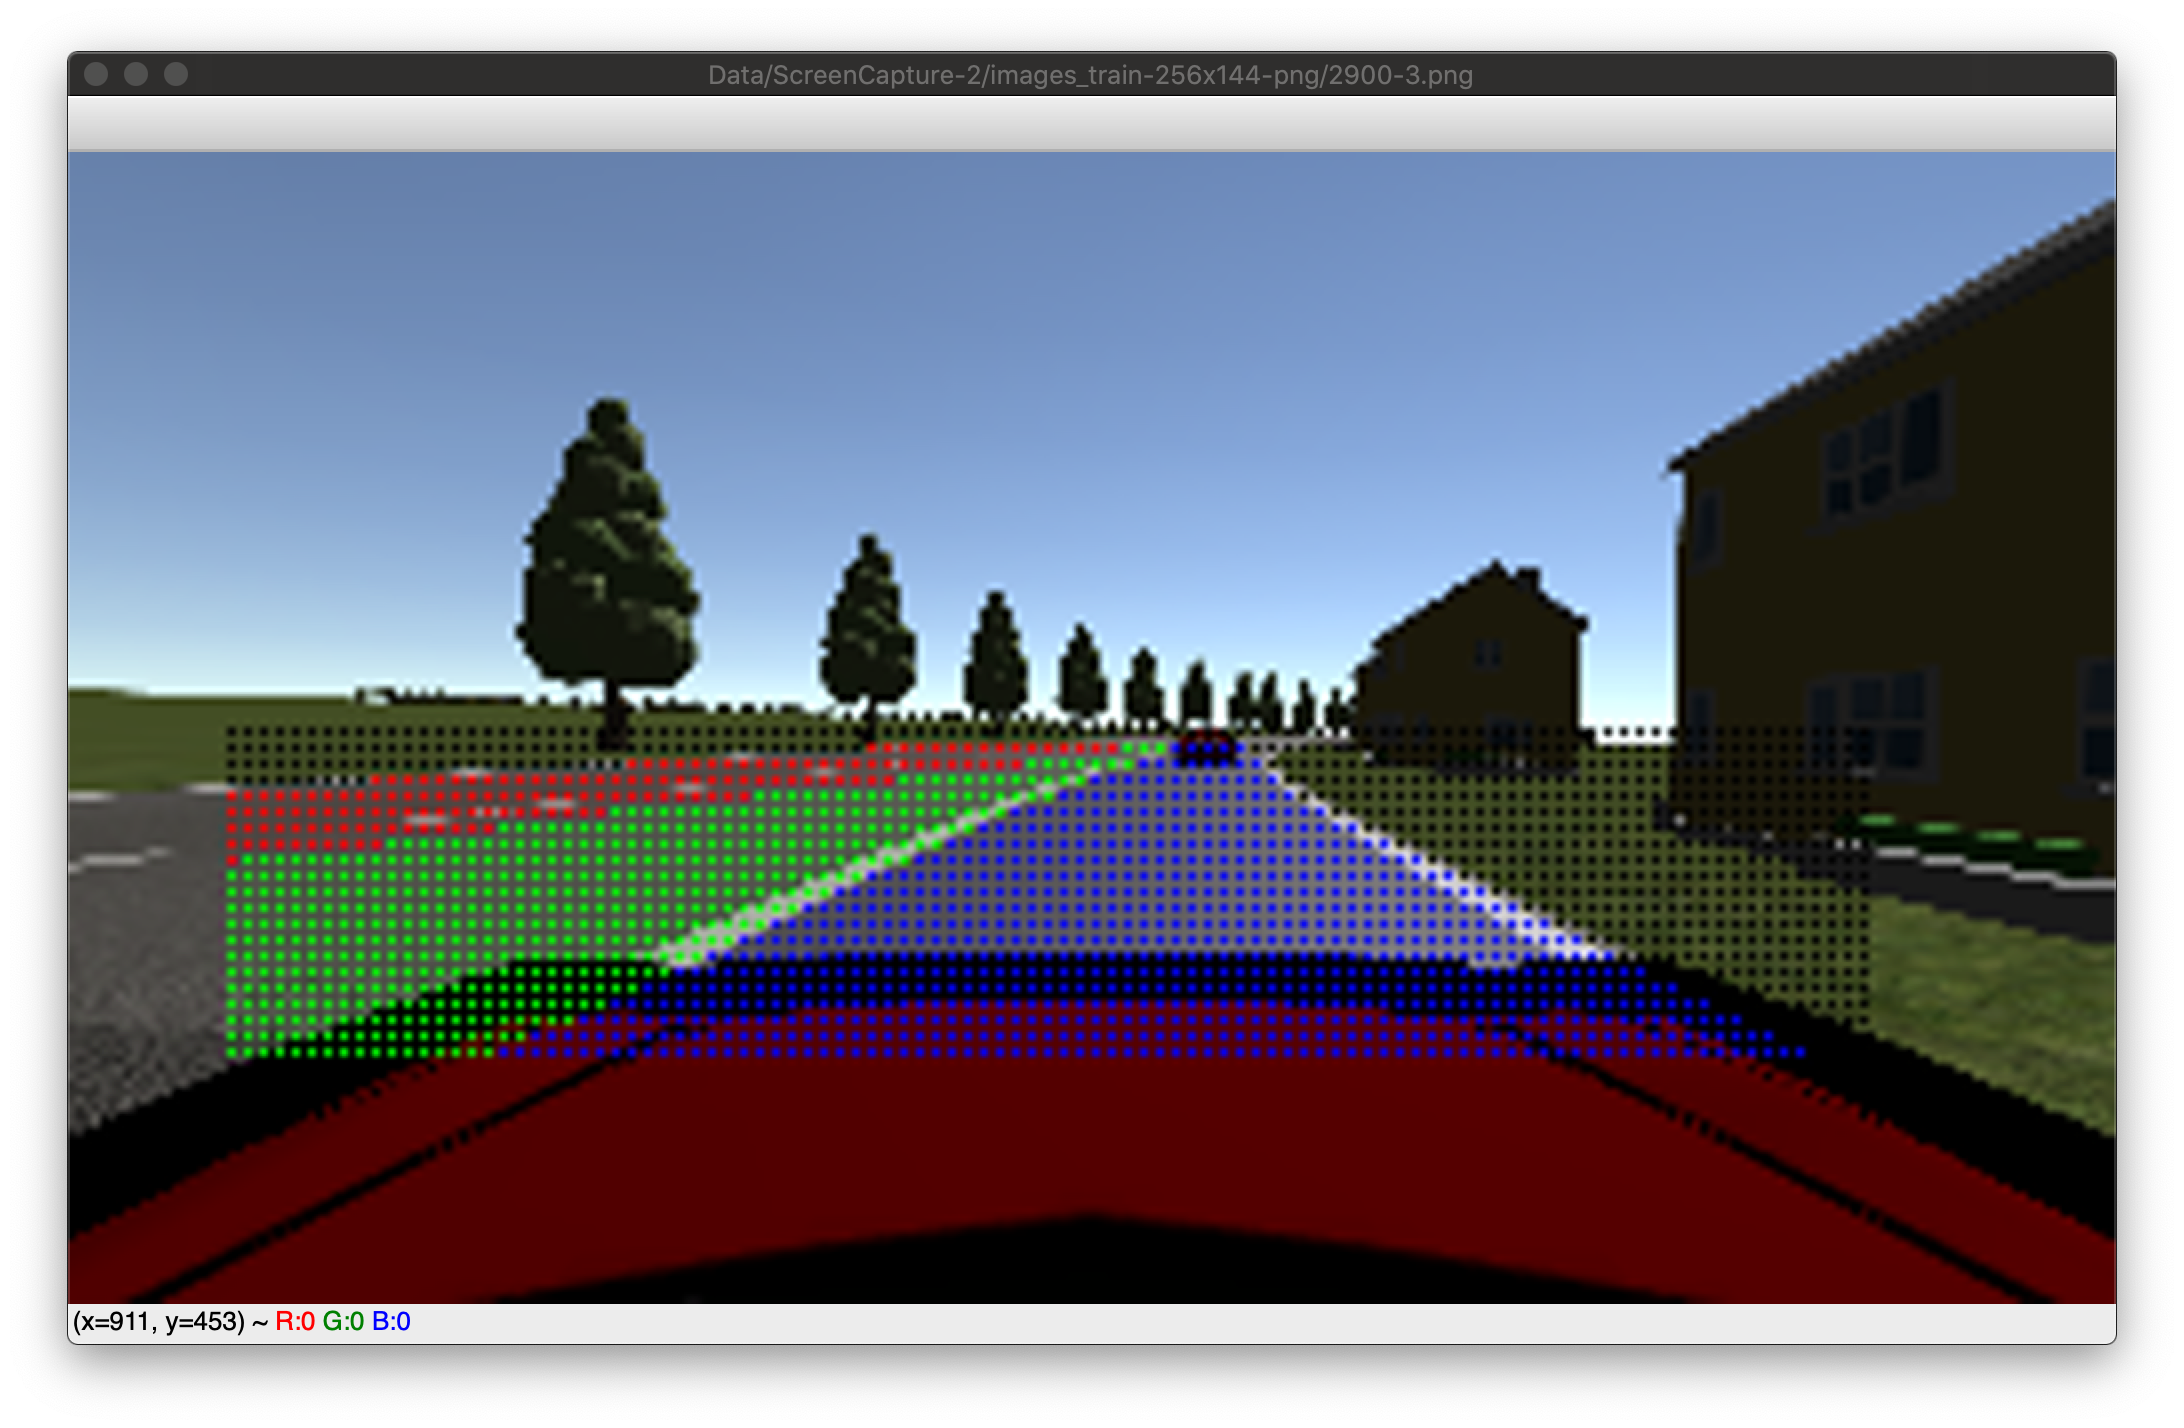
\includegraphics[scale=0.31]{images/Chapter5/lane3-curve-green.png}
  \caption{Good results on curved 3-lane highway}
  \label{fig:good-curve-3}
\end{figure}
\begin{figure}[H]
  \centering
  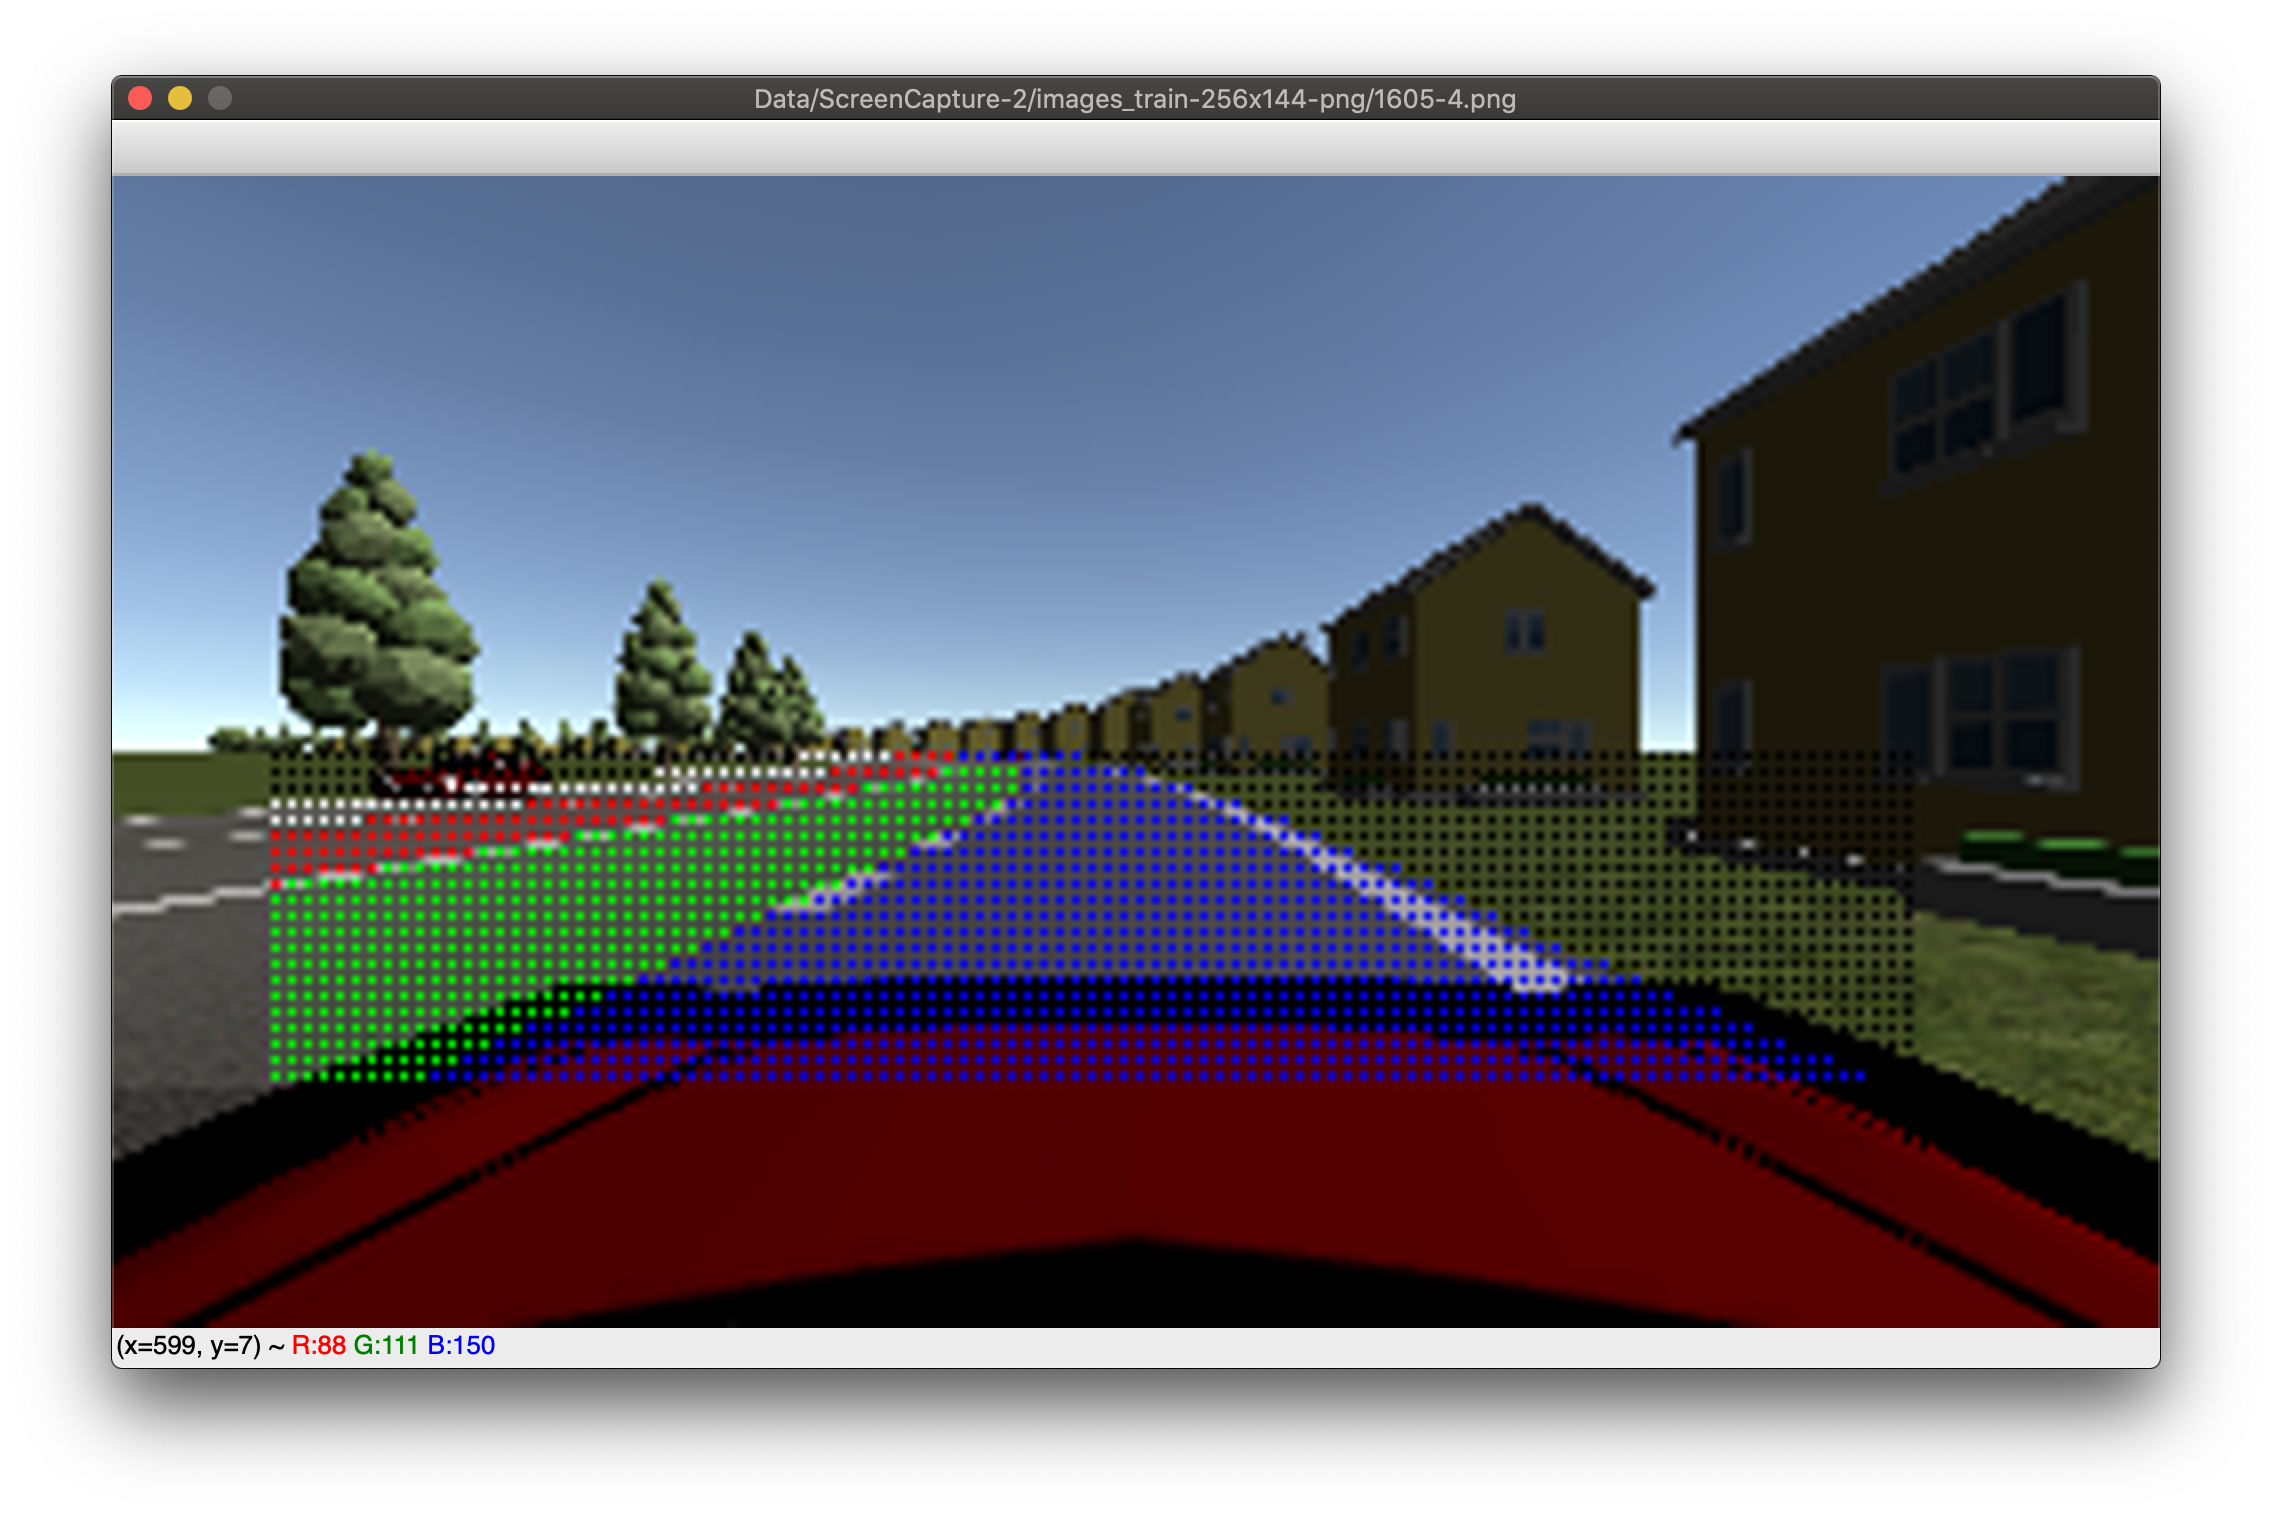
\includegraphics[scale=0.31]{images/Chapter5/lane4-curve-green.png}
  \caption{Good results on curved 4-lane highway}
  \label{fig:good-curve-4}
\end{figure}

\par
The Figures \ref{fig:red-1}, \ref{fig:red-2}, \ref{fig:red-3} and \ref{fig:red-4} shows that predictions on some images were very totally incorrect. This is mostly because the model classified the scene having different number of maximum lanes.
\begin{figure}[H]
  \centering
  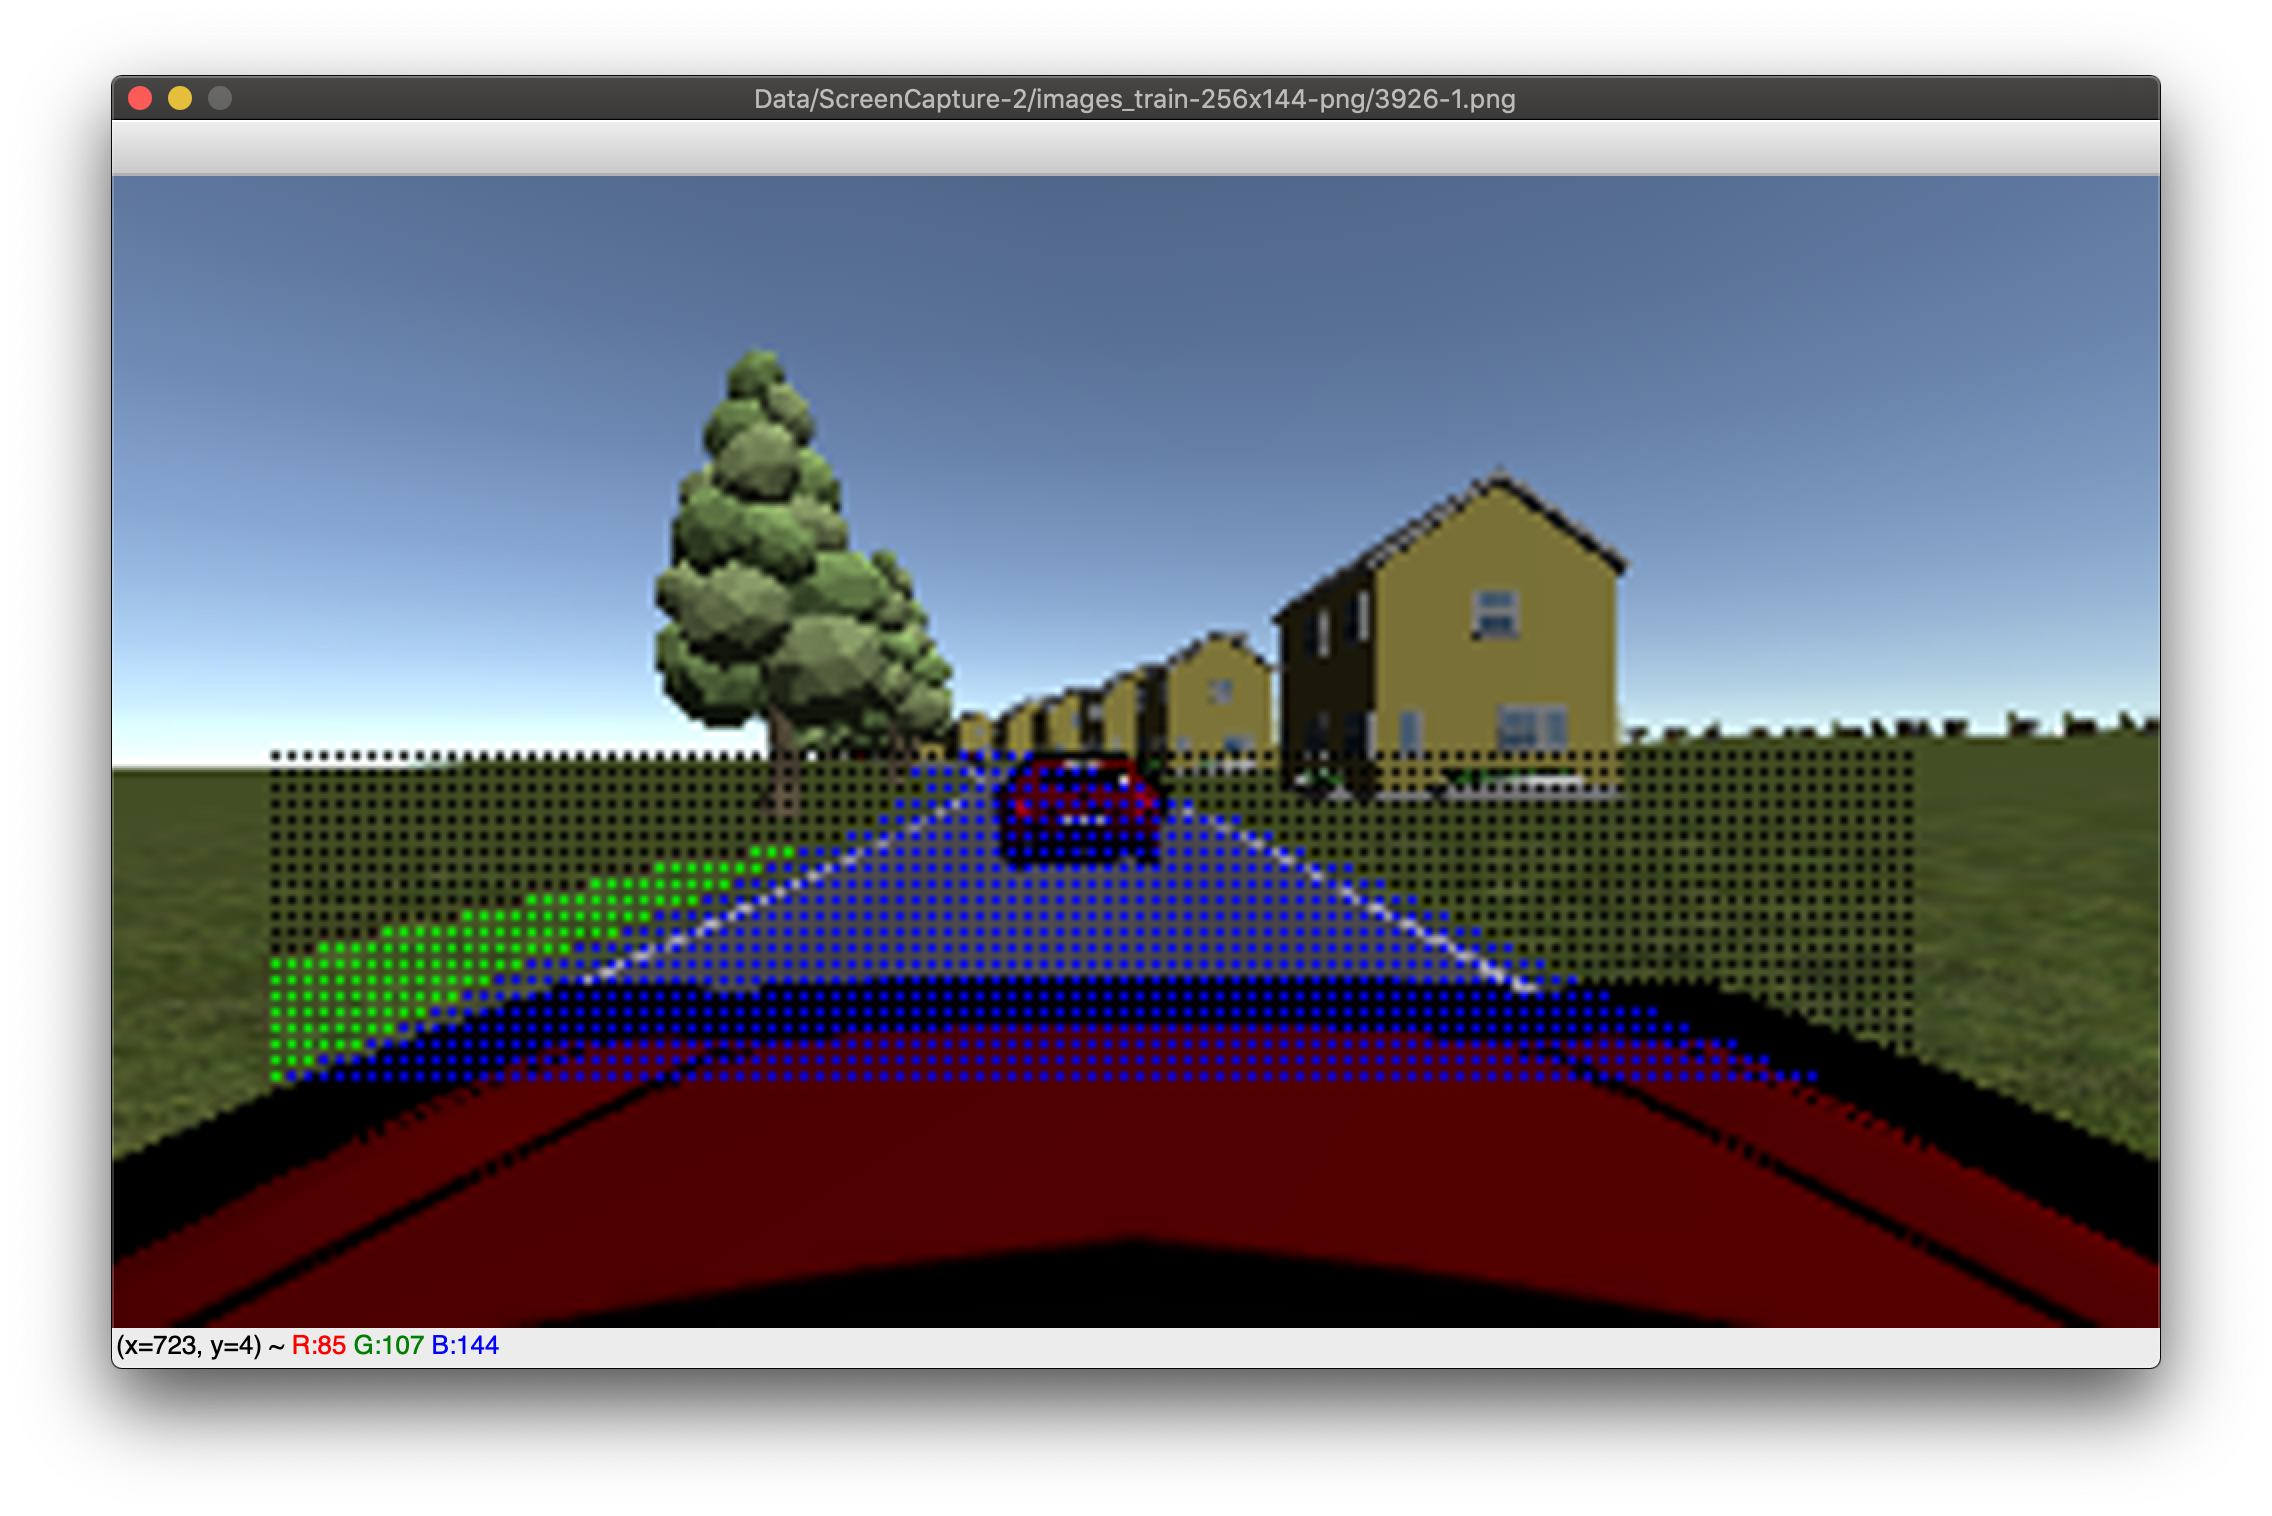
\includegraphics[scale=0.31]{images/Chapter5/lane1-red.png}
  \caption{Classified 1-lane highway as 2-lane highway}
  \label{fig:red-1}
\end{figure}
\begin{figure}[H]
  \centering
  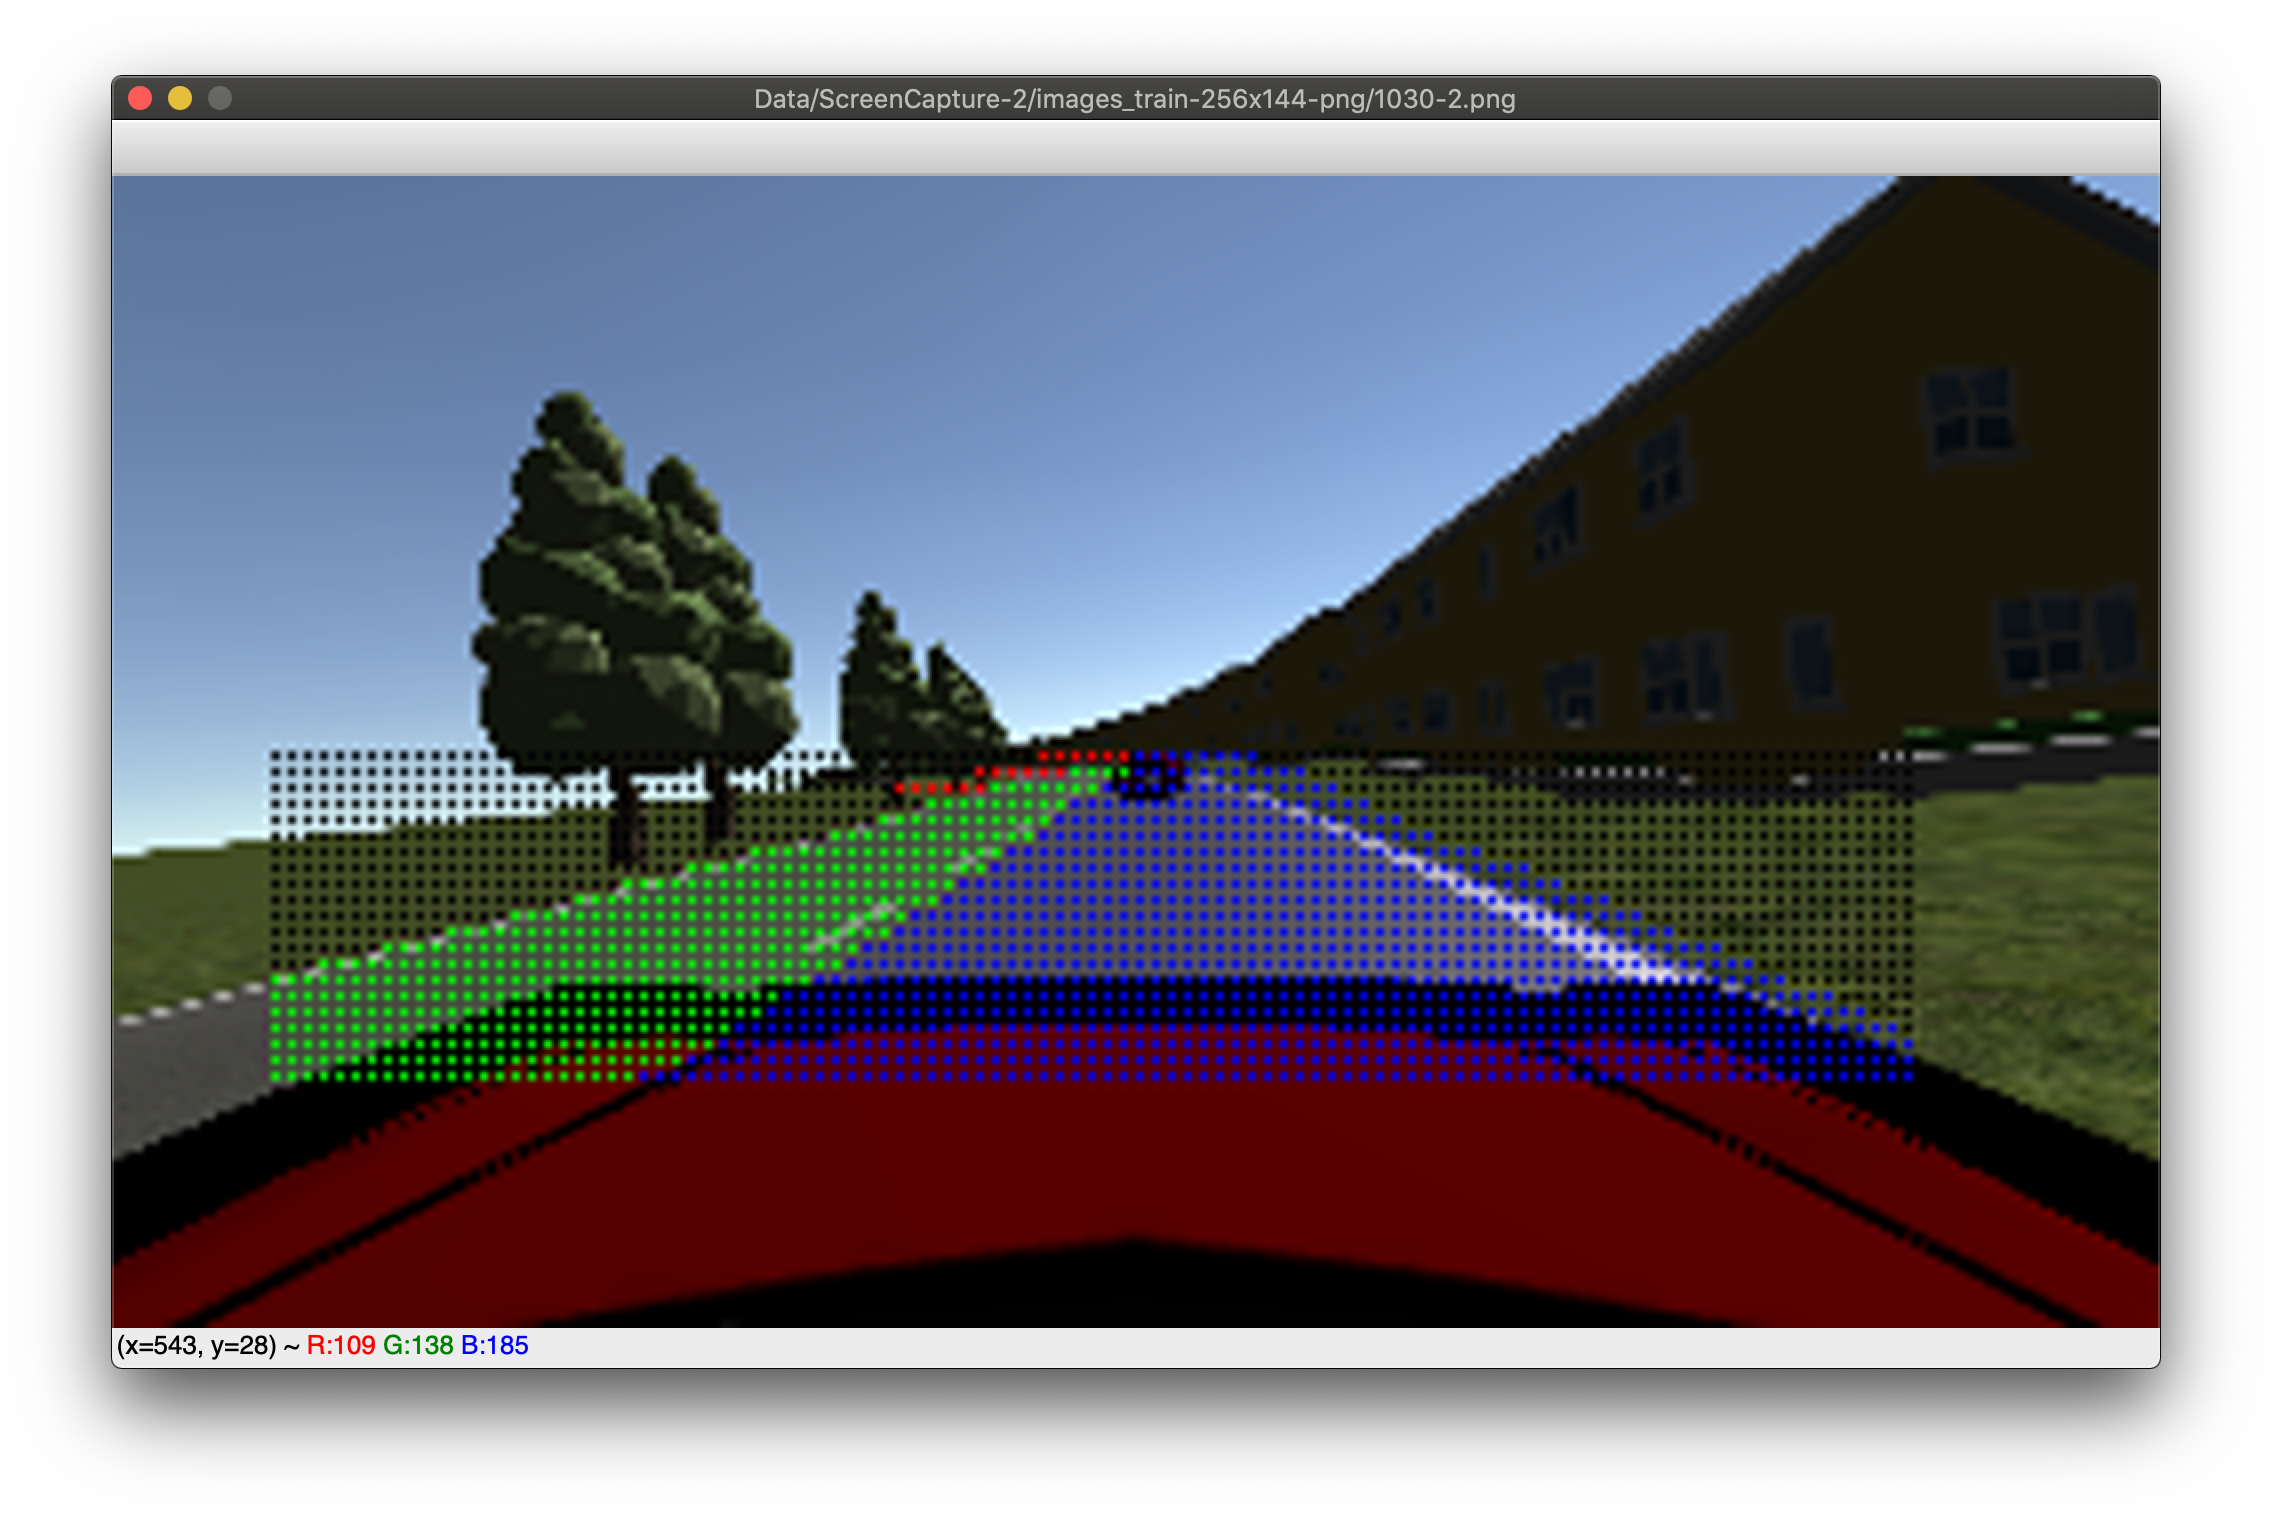
\includegraphics[scale=0.31]{images/Chapter5/lane2-red.png}
  \caption{Classified 2-lane highway as 3-lane highway}
  \label{fig:red-2}
\end{figure}
\begin{figure}[H]
  \centering
  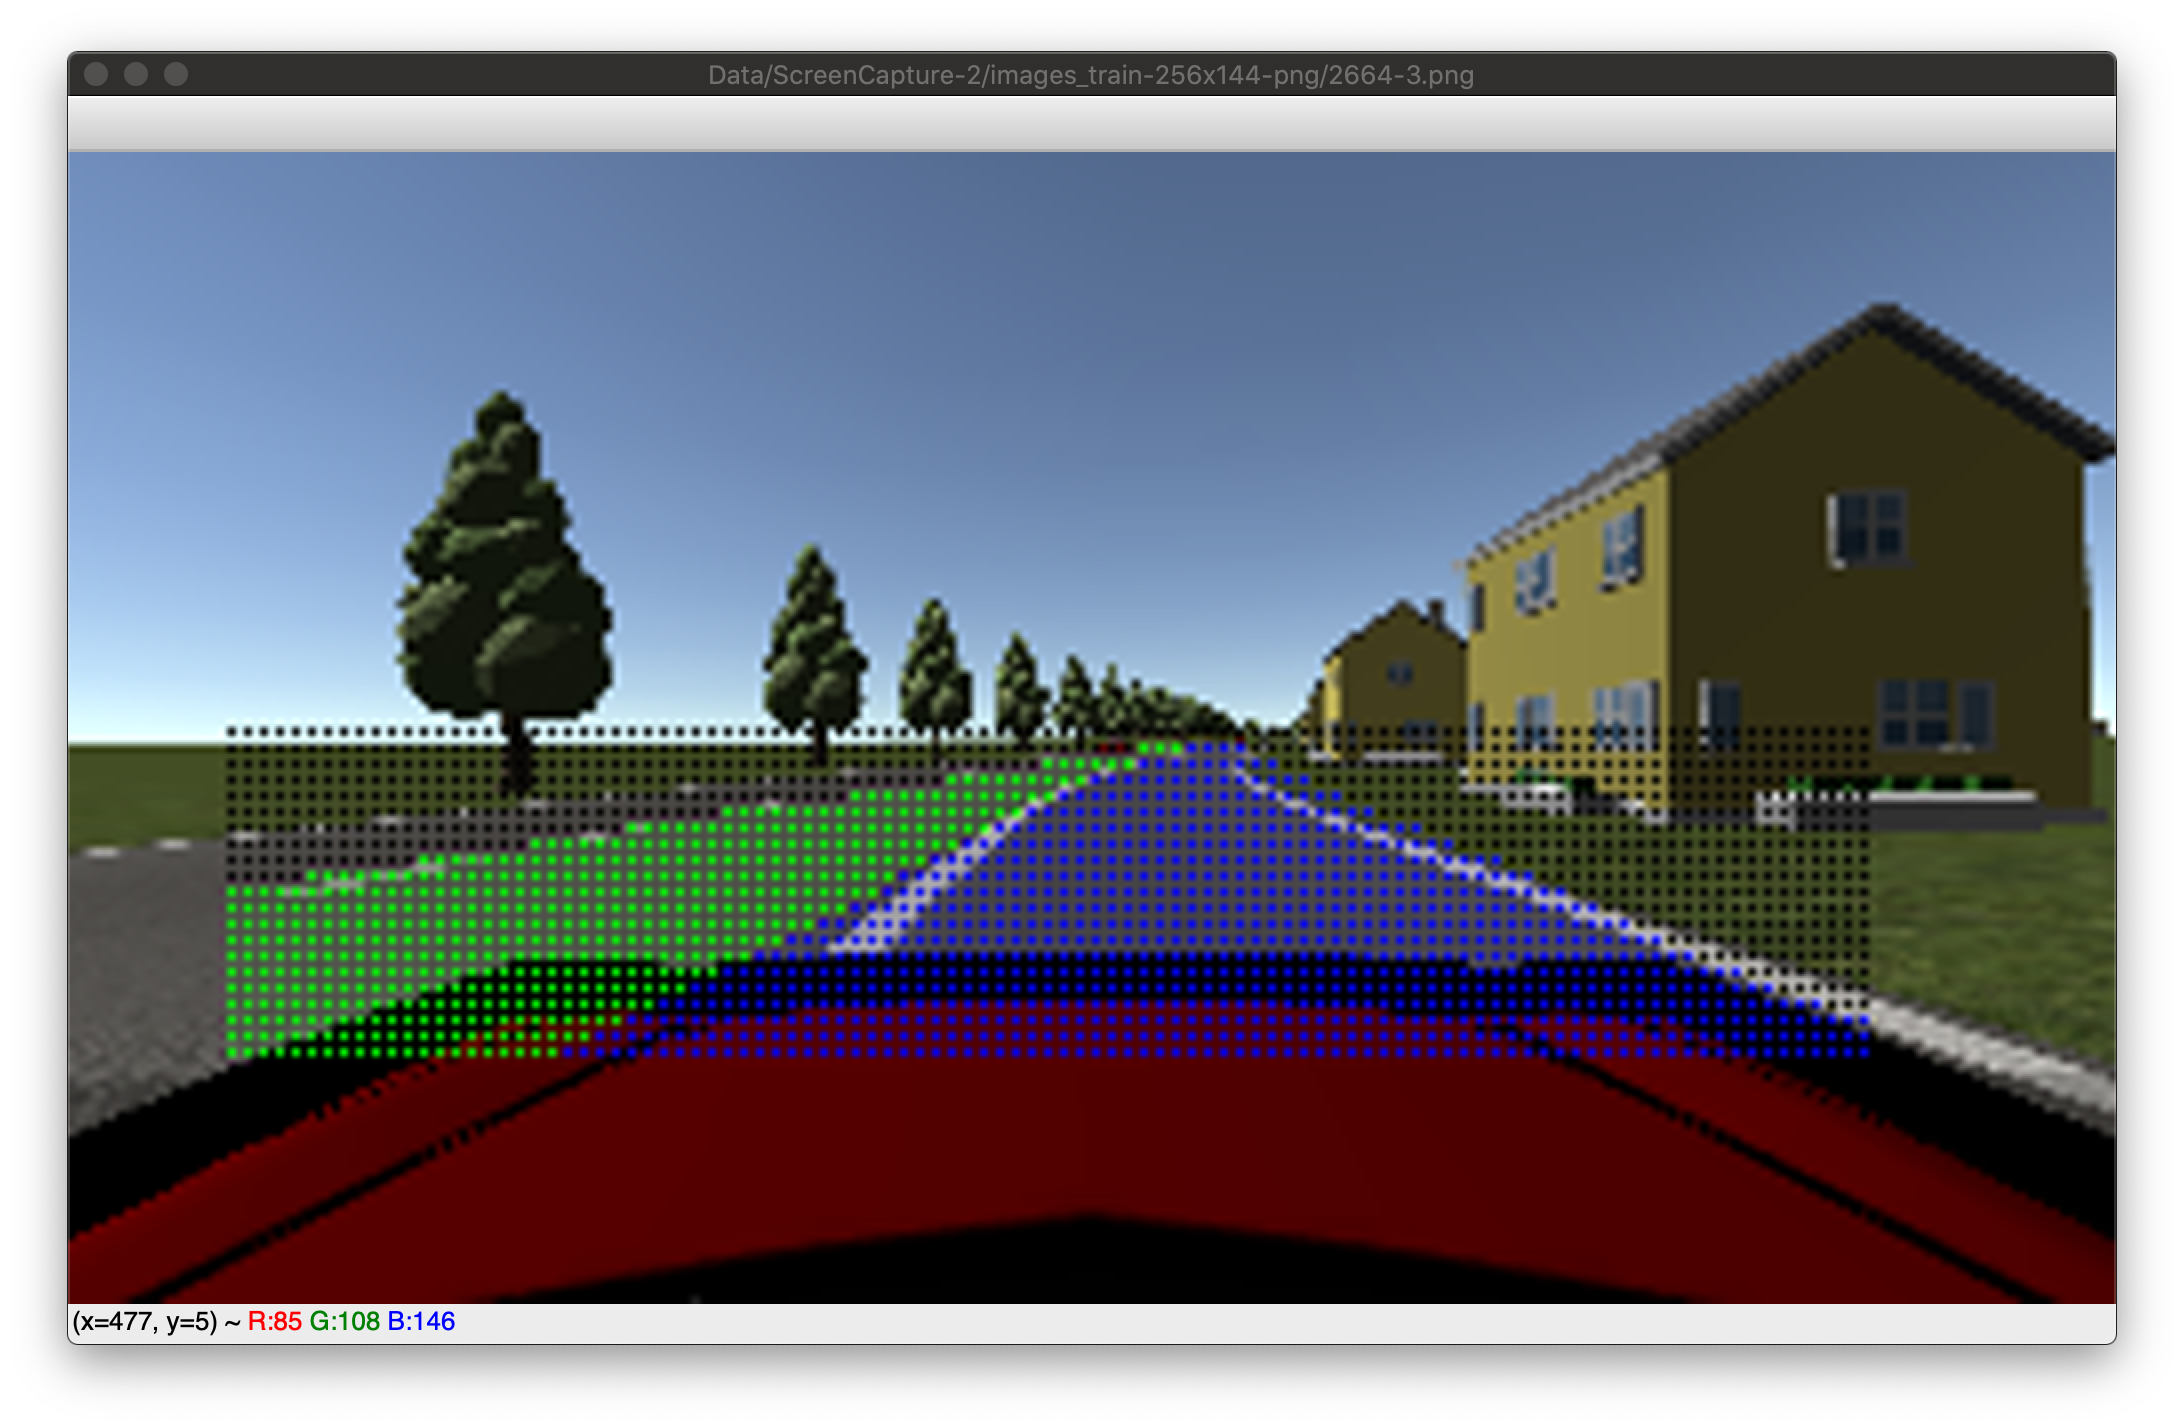
\includegraphics[scale=0.31]{images/Chapter5/lane3-red.png}
  \caption{Classified 3-lane highway as 2-lane highway}
  \label{fig:red-3}
\end{figure}
\begin{figure}[H]
  \centering
  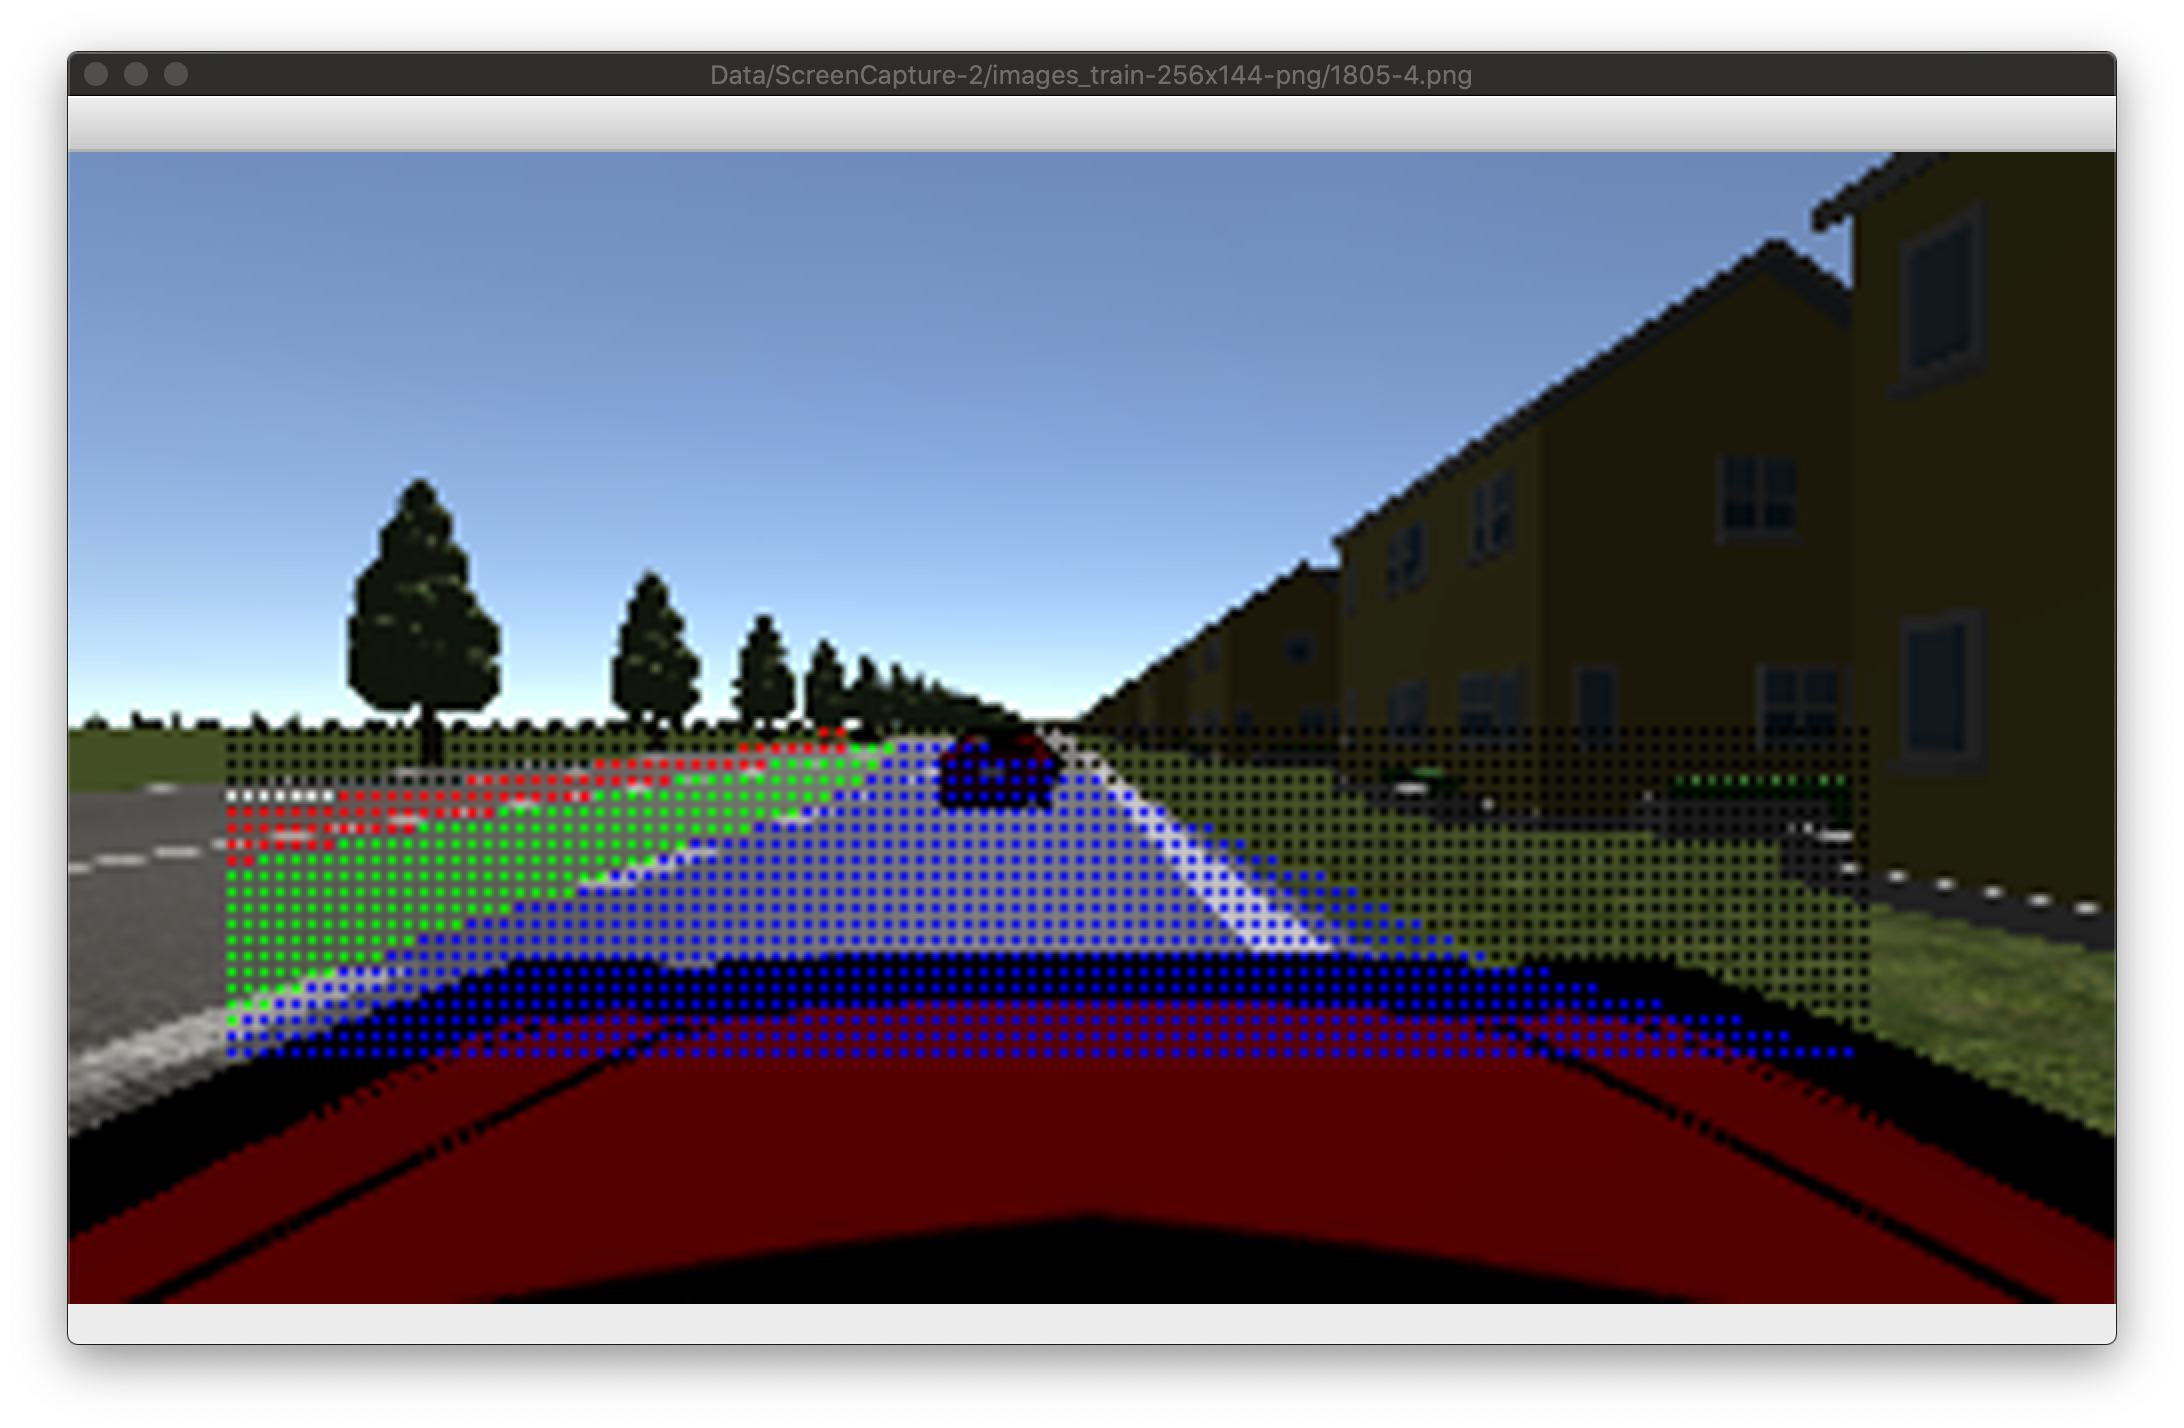
\includegraphics[scale=0.31]{images/Chapter5/lane4-red.png}
  \caption{Classified 4-lane highway as 3-lane highway}
  \label{fig:red-4}
\end{figure}

% The Figures \ref{fig:yellow-1}, \ref{fig:yellow-2}, \ref{fig:yellow-3} and \ref{fig:yellow-4} shows that predictions on some images were very totally incorrect. even though the model classified the scene having same number of maximum lanes.
% \begin{figure}[H]
%   \centering
%   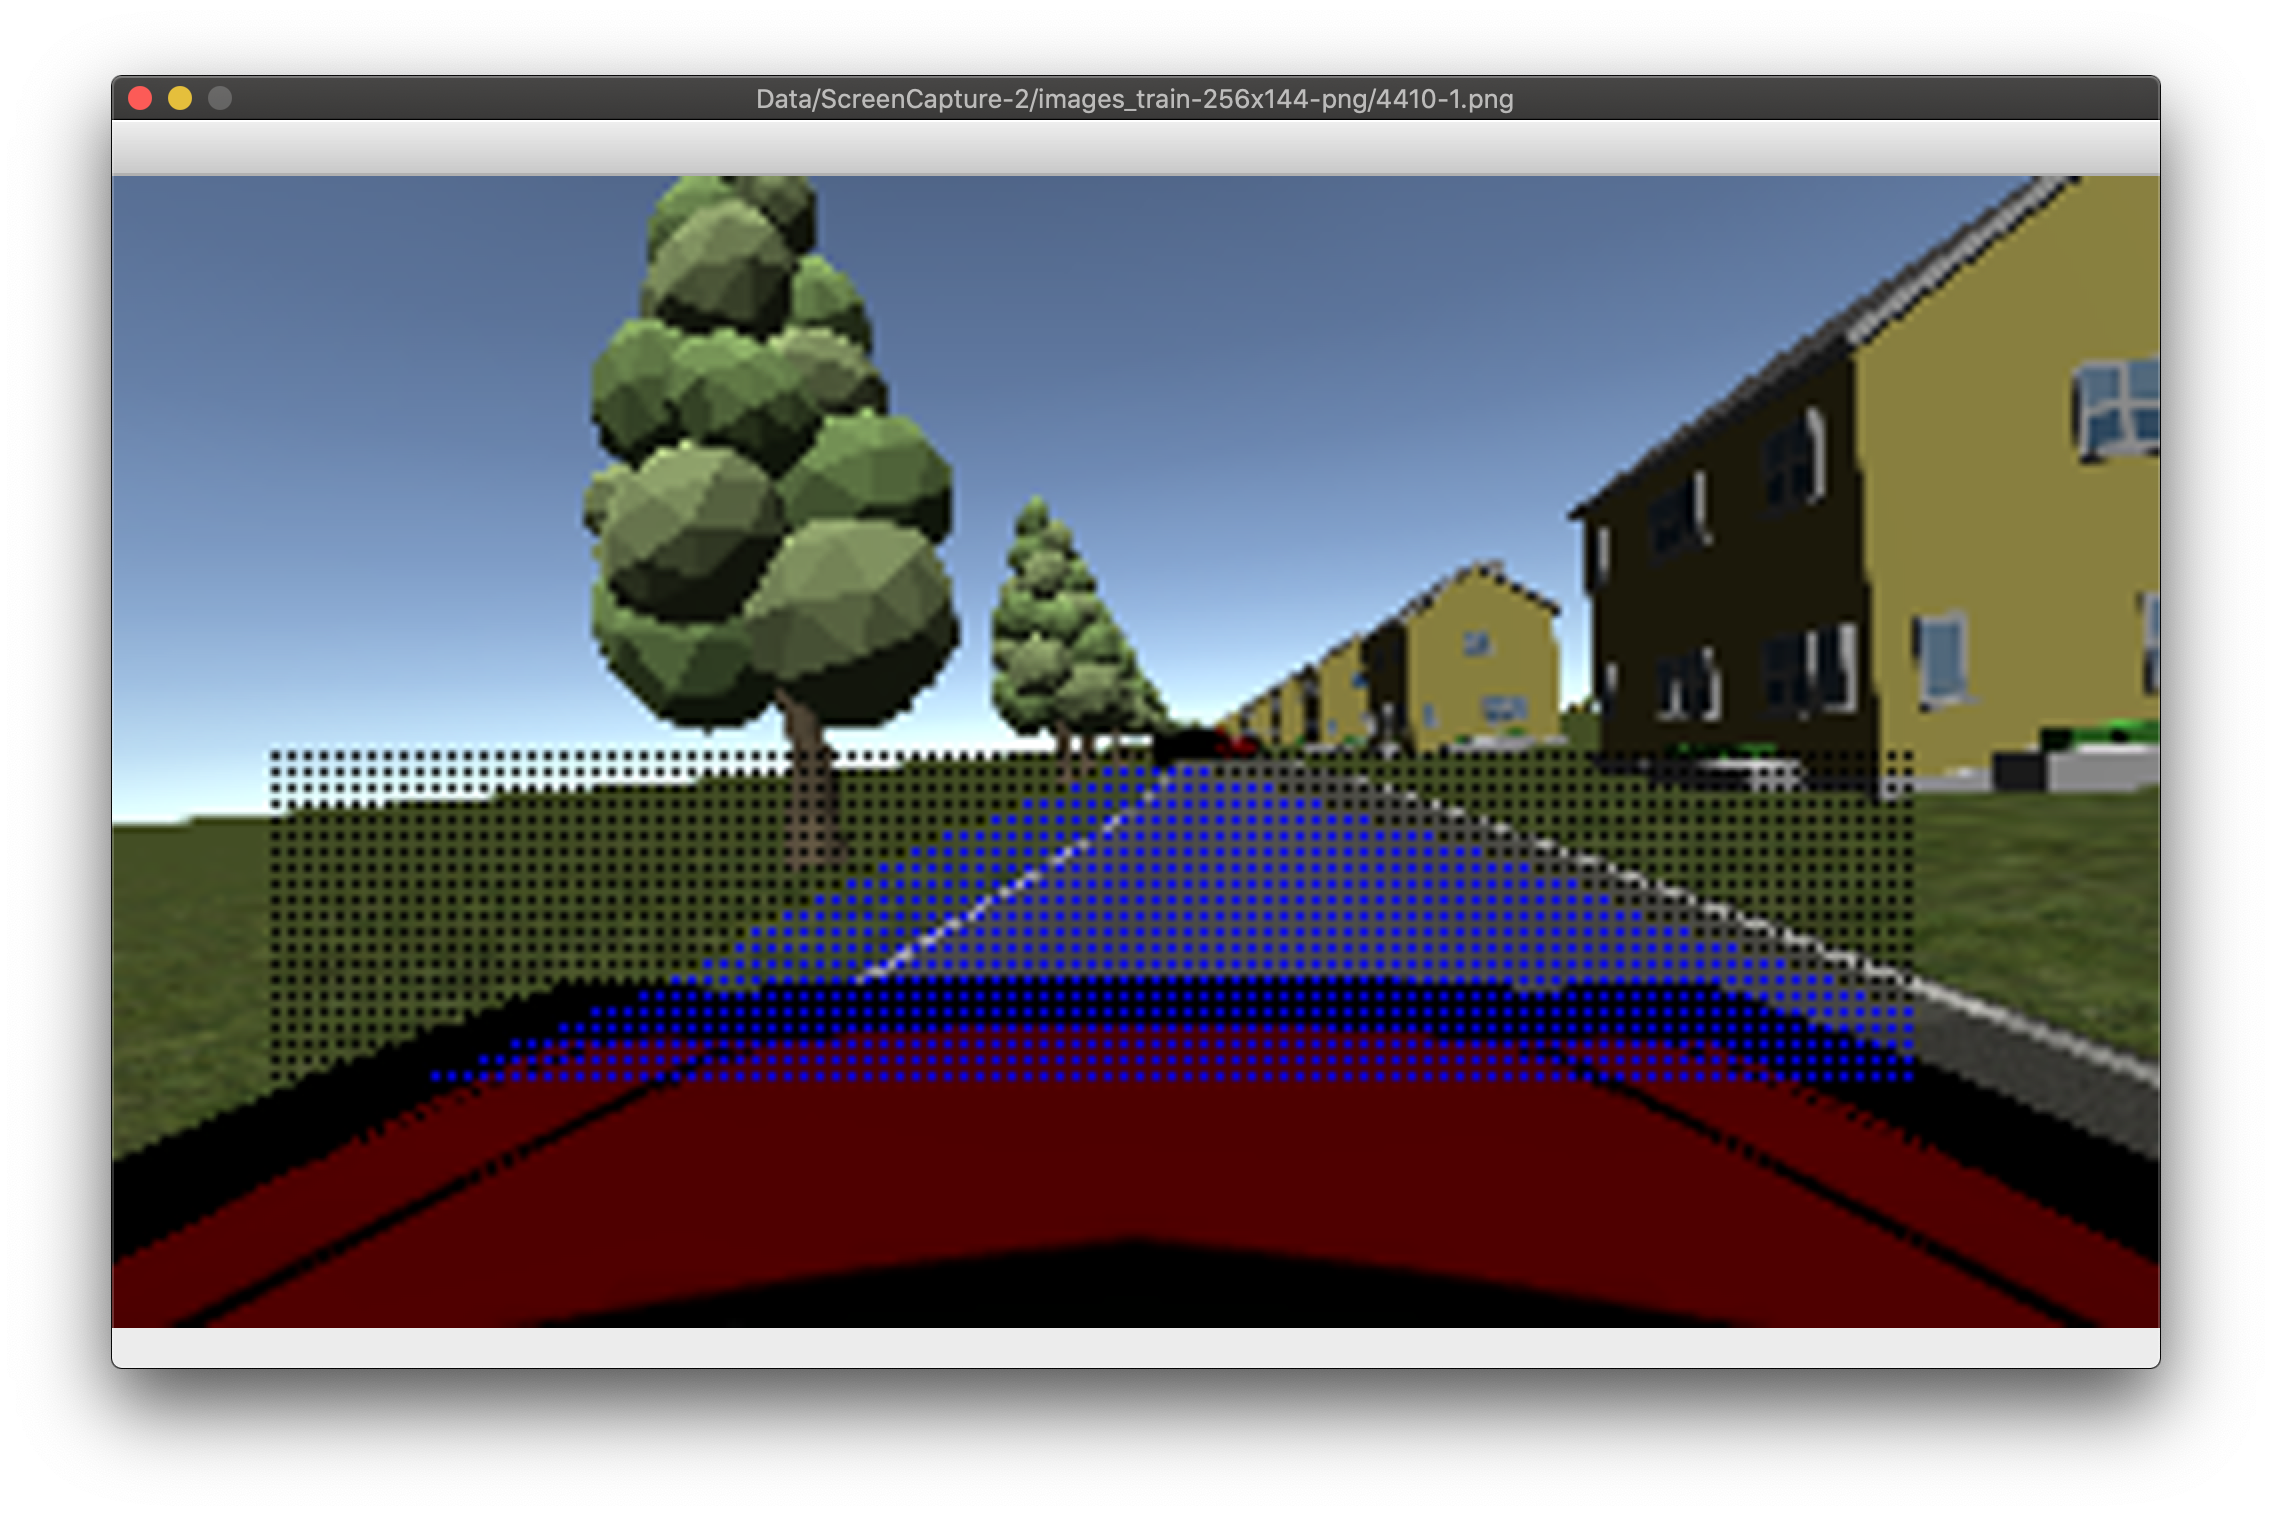
\includegraphics[scale=0.31]{images/Chapter5/lane1-yellow.png}
%   \caption{Some incorrect point predictions on 1-lane highway}
%   \label{fig:yellow-1}
% \end{figure}
% \begin{figure}[H]
%   \centering
%   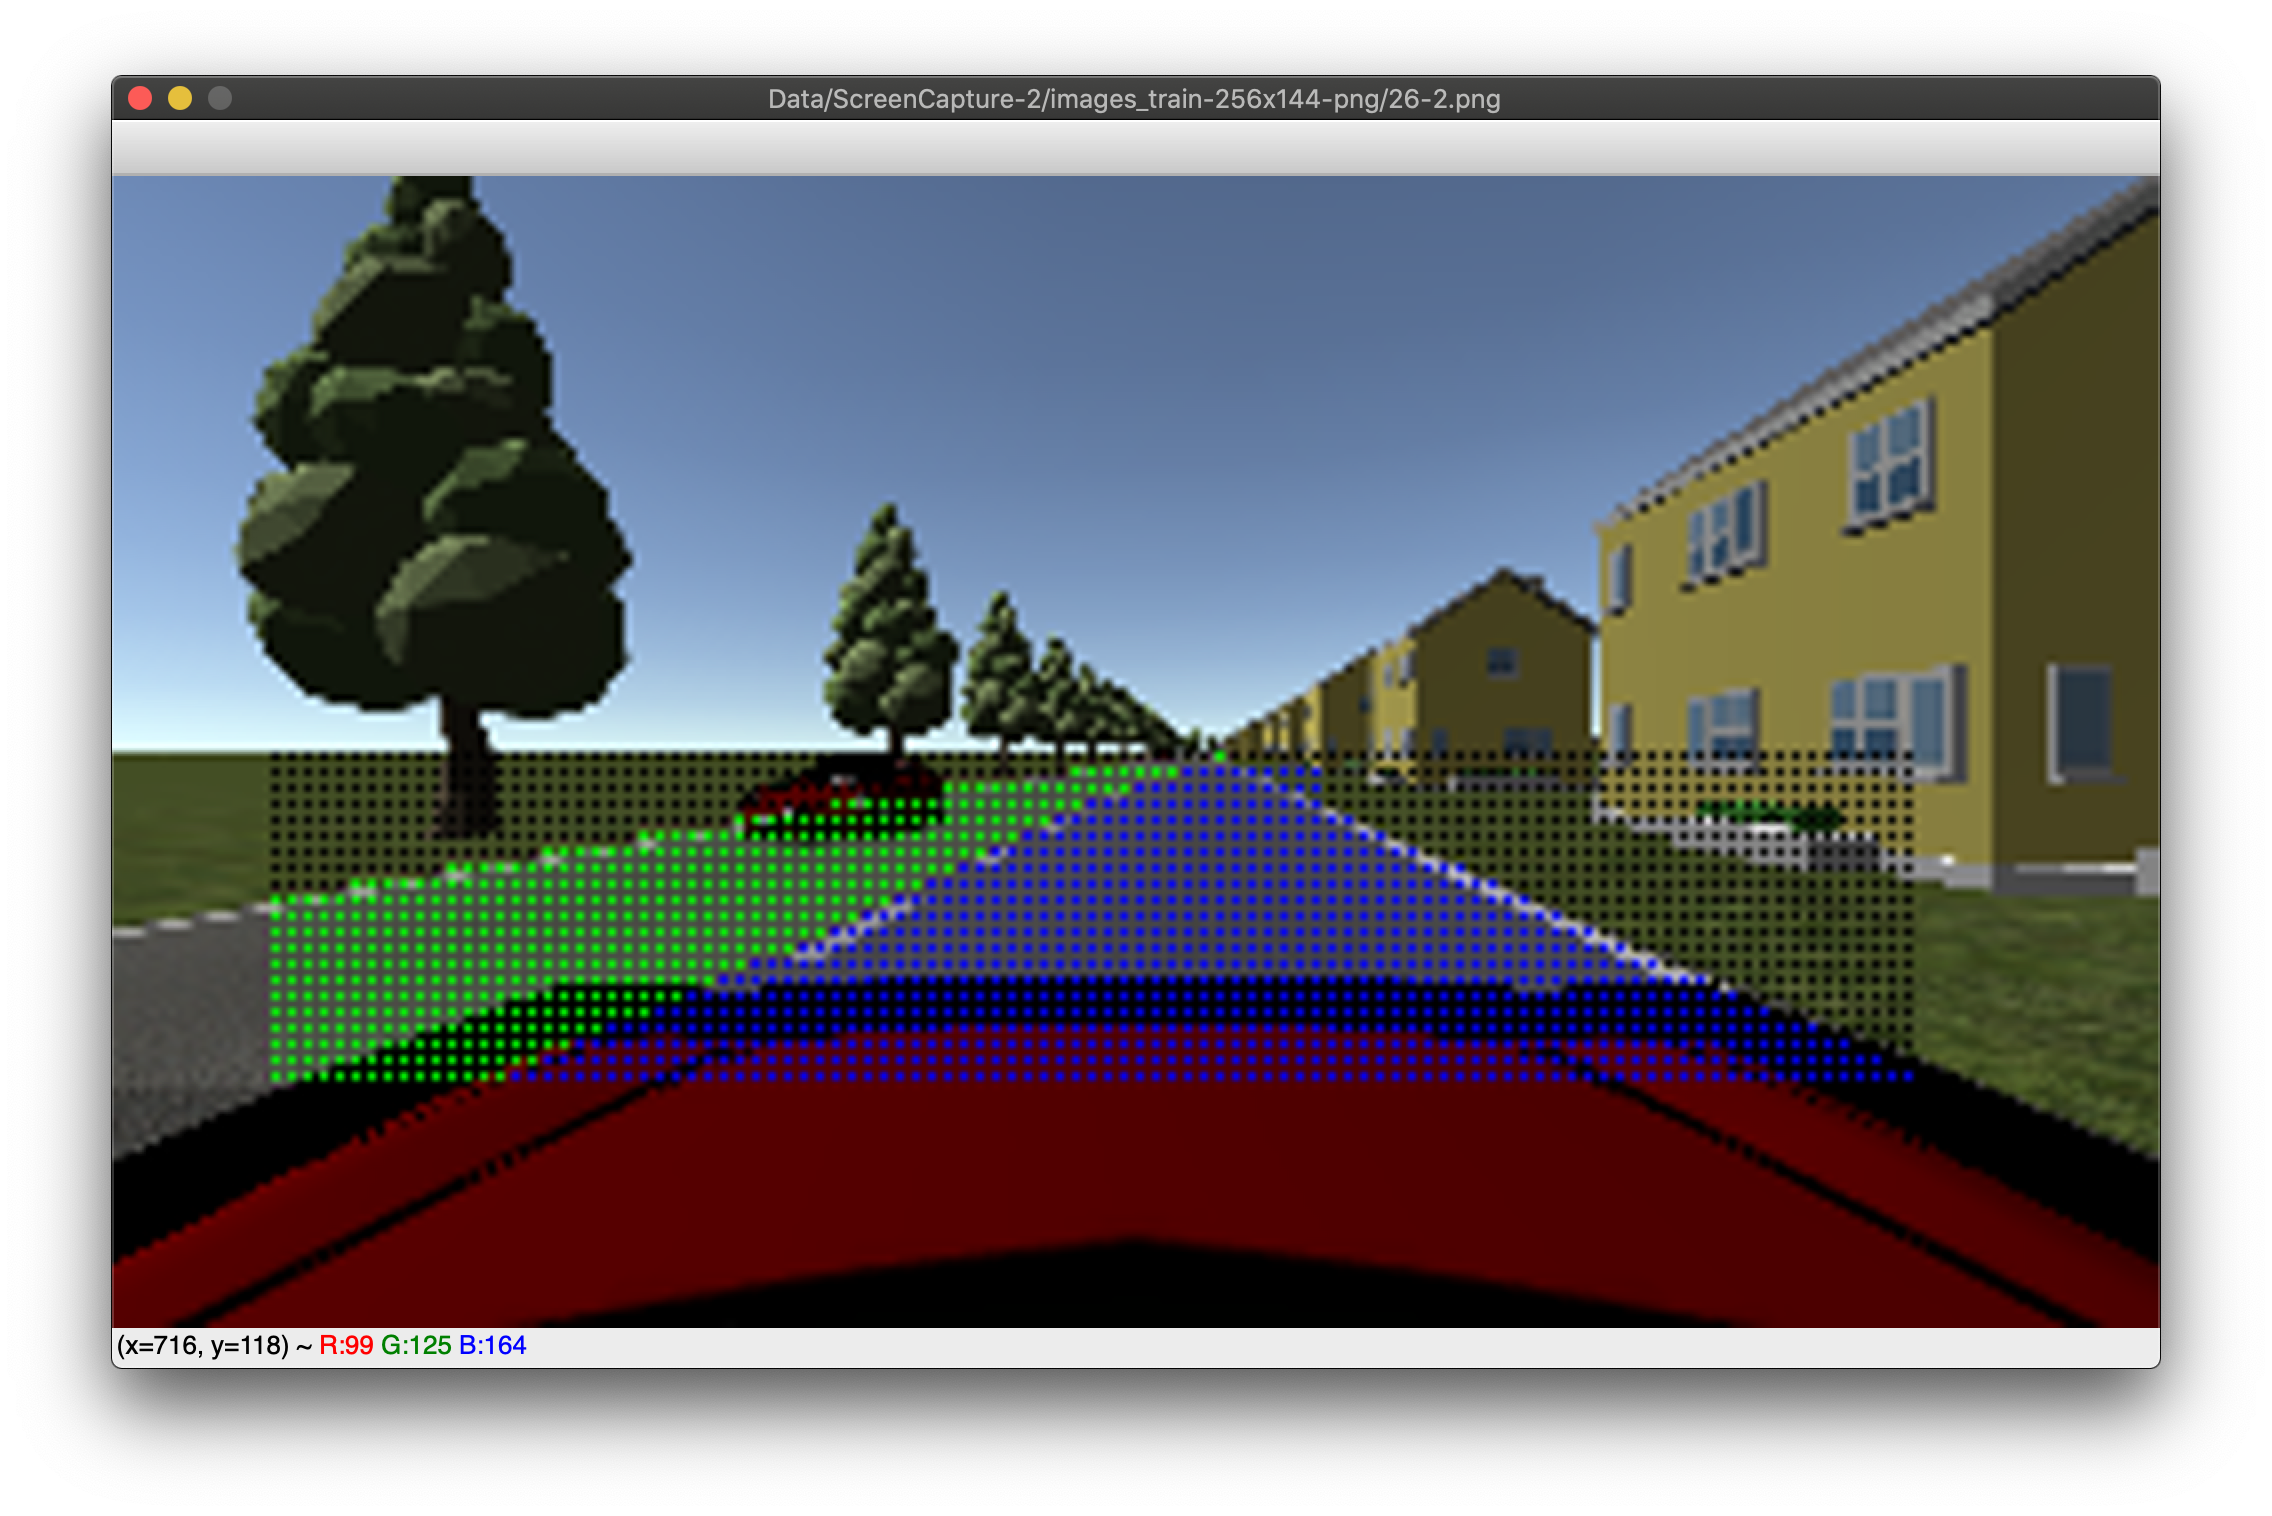
\includegraphics[scale=0.31]{images/Chapter5/lane2-yellow.png}
%   \caption{Some incorrect point predictions on 2-lane highway}
%   \label{fig:yellow-2}
% \end{figure}
% \begin{figure}[H]
%   \centering
%   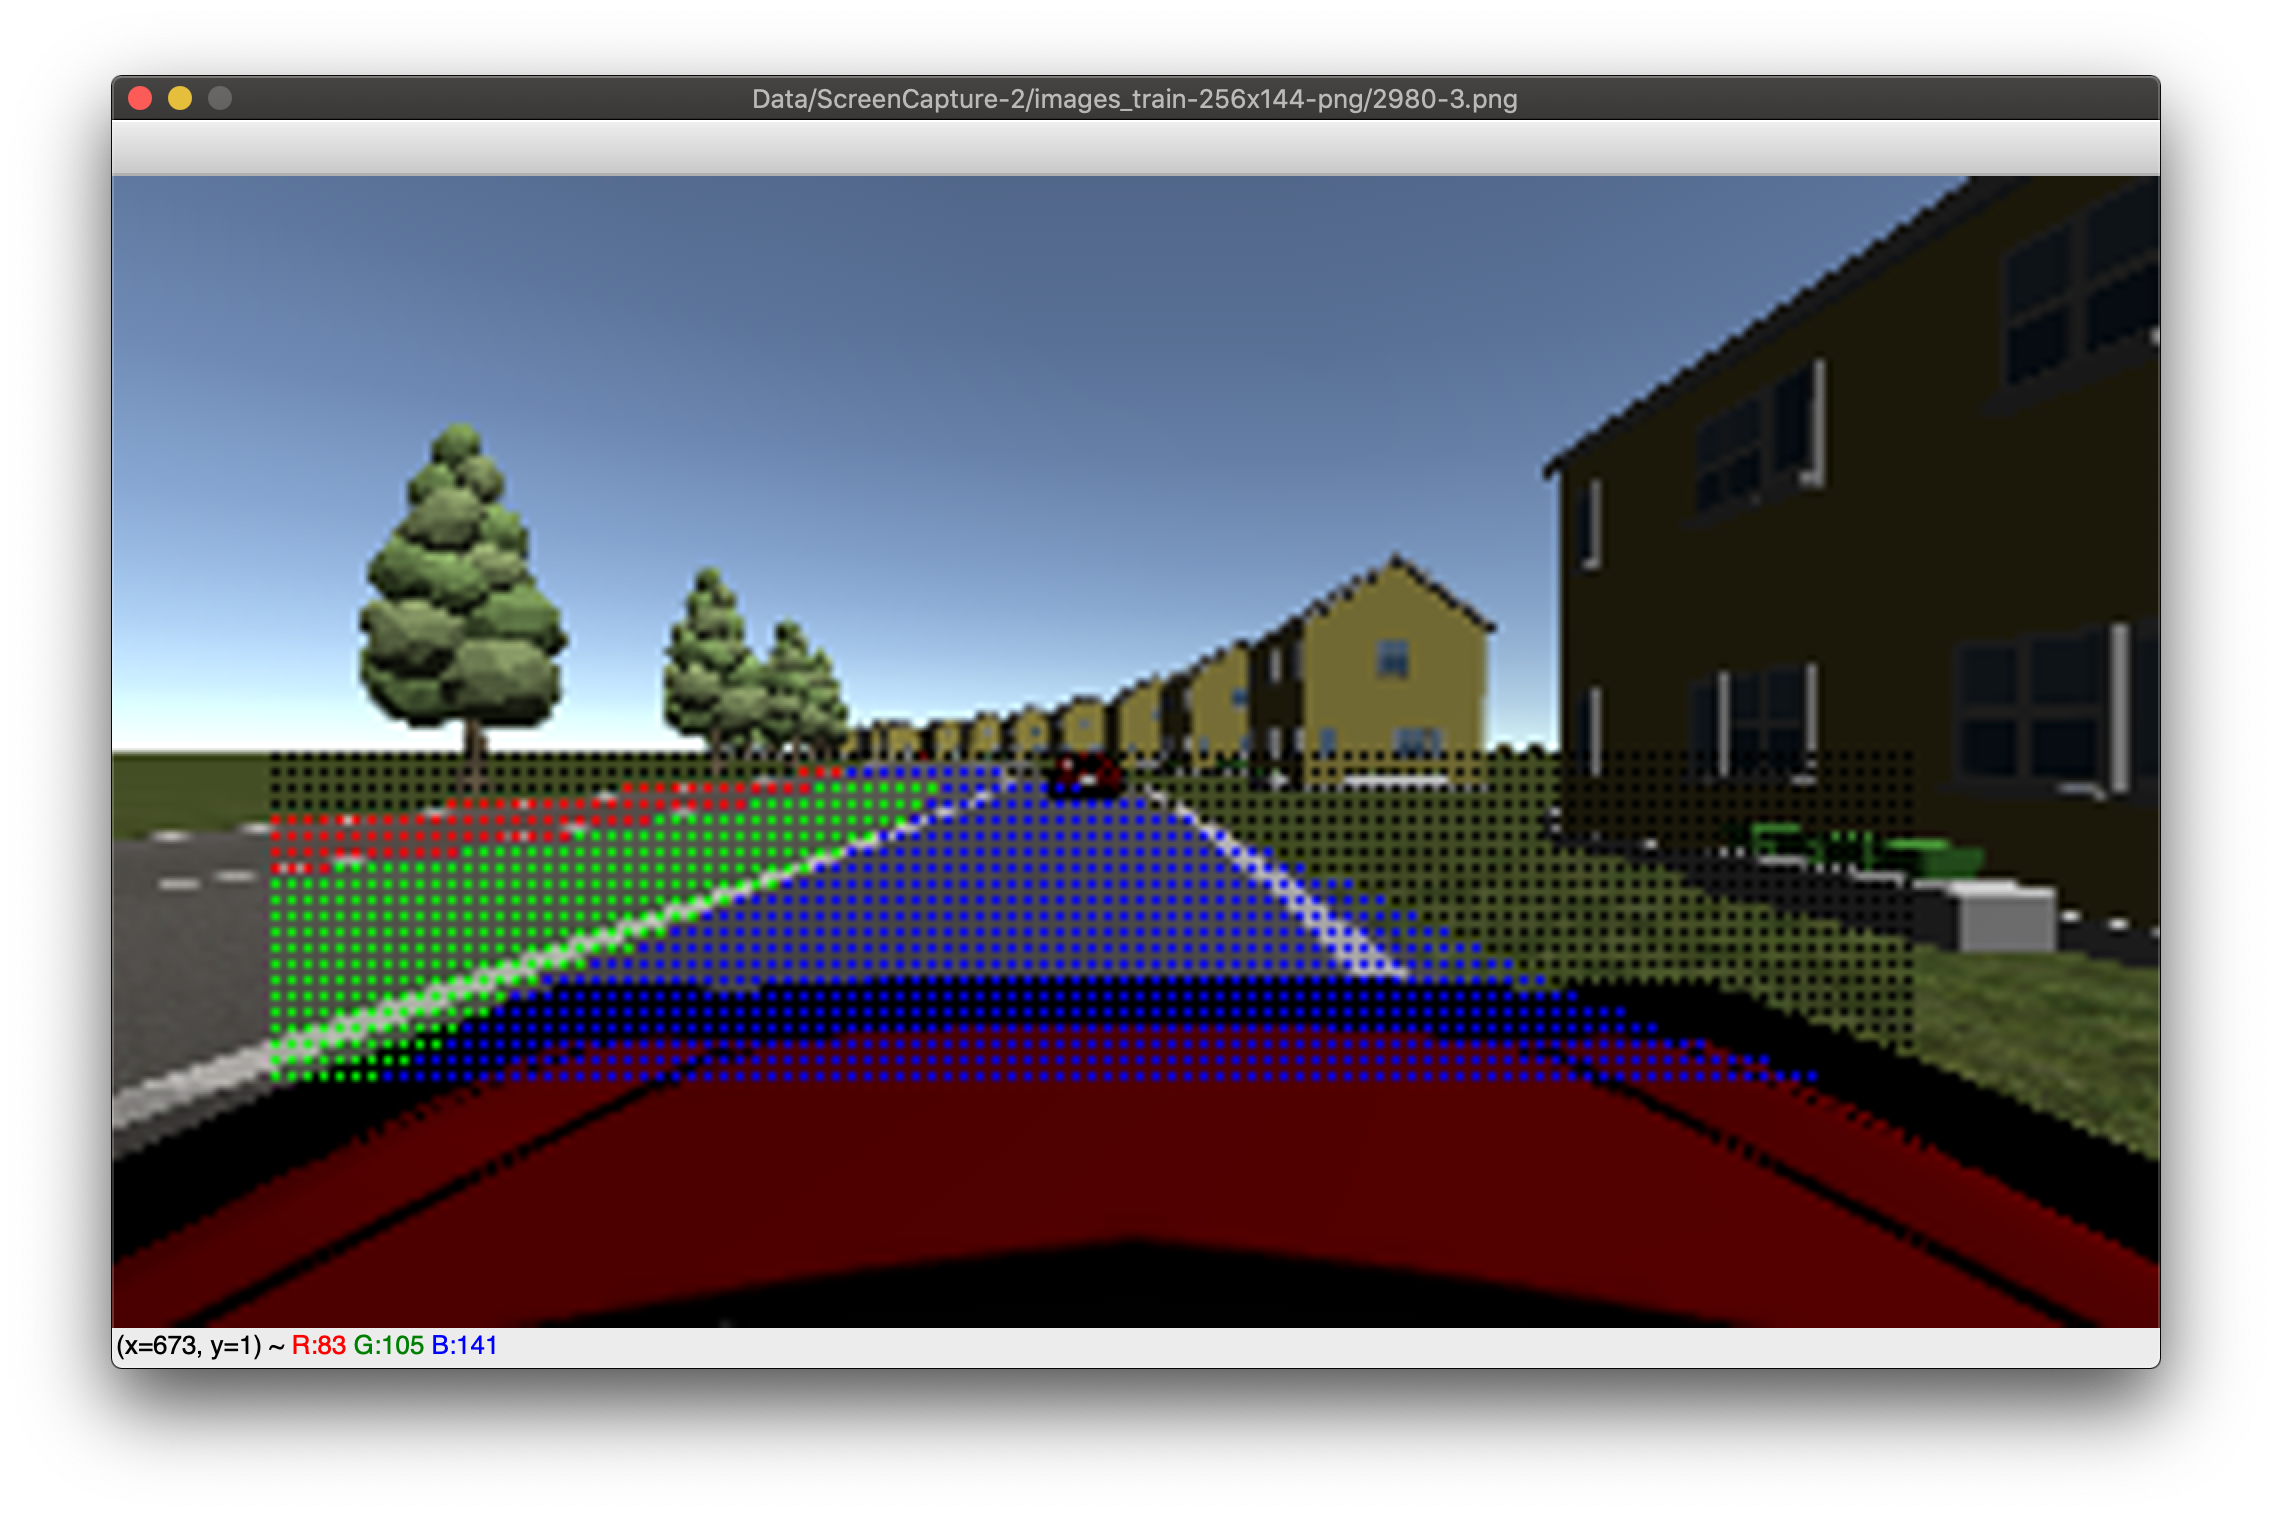
\includegraphics[scale=0.31]{images/Chapter5/lane3-yellow.png}
%   \caption{Some incorrect point predictions on 3-lane highway}
%   \label{fig:yellow-3}
% \end{figure}
% \begin{figure}[H]
%   \centering
%   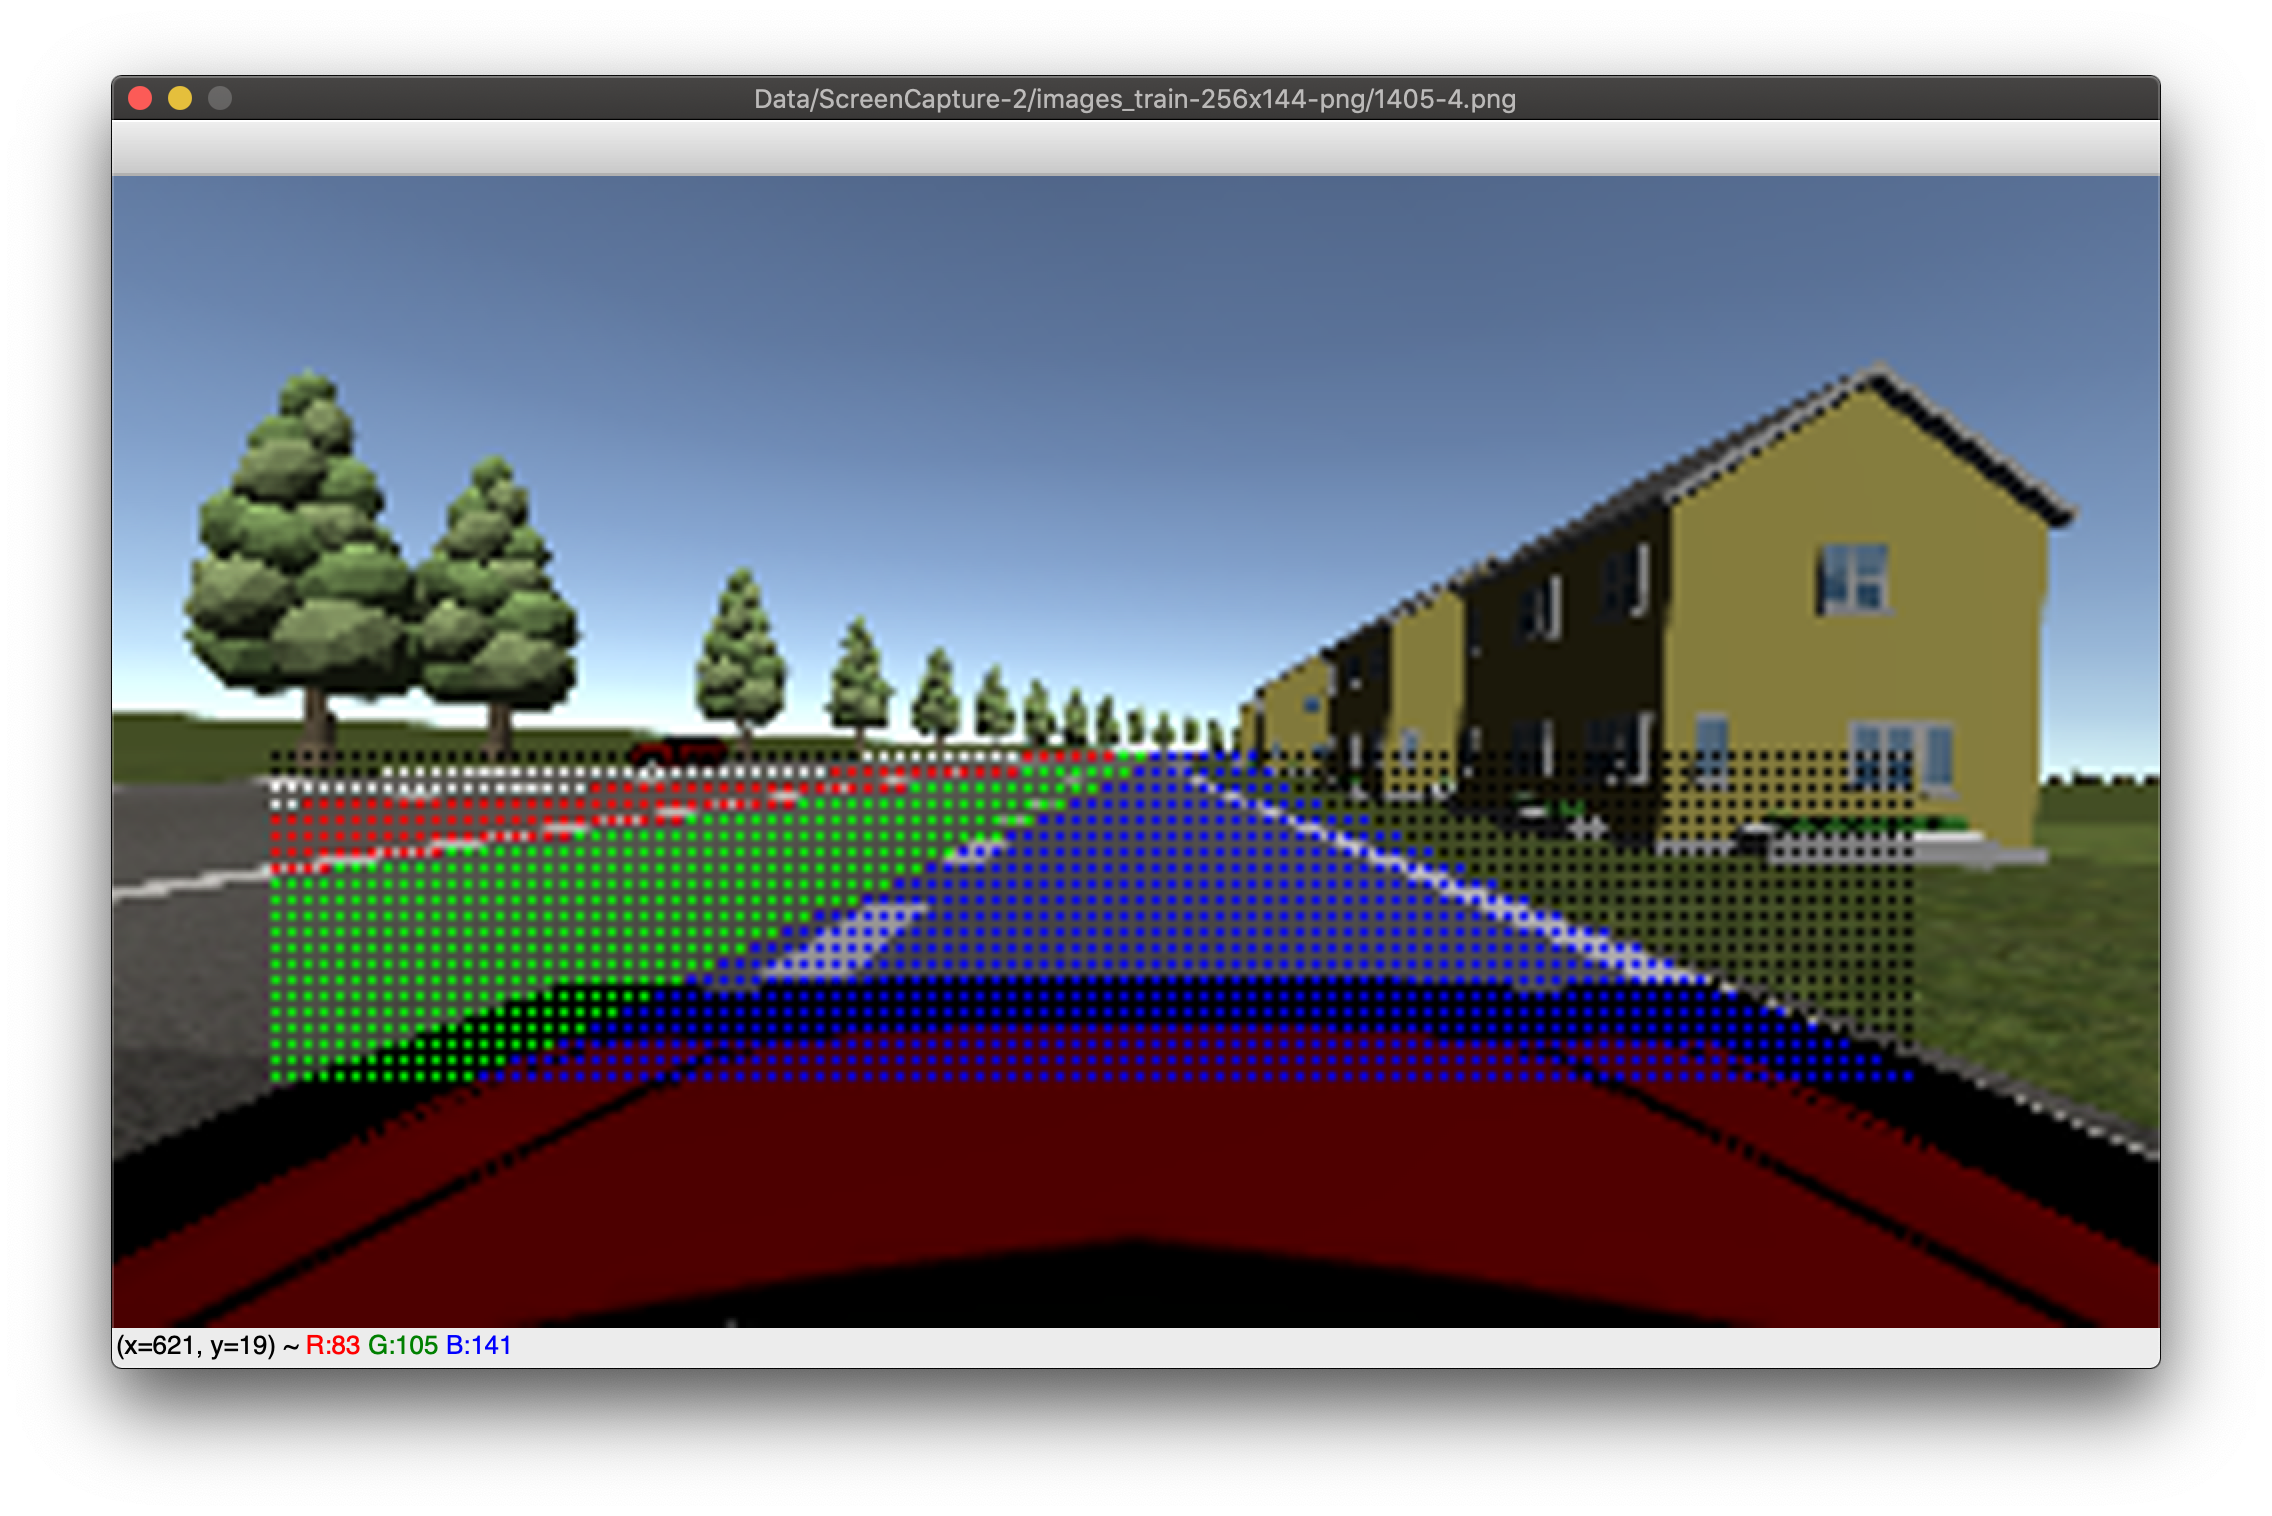
\includegraphics[scale=0.31]{images/Chapter5/lane4-yellow.png}
%   \caption{Some incorrect point predictions on 4-lane highway}
%   \label{fig:yellow-4}
% \end{figure}



% \begin{figure}[H]
%   \centering
% 	\begin{subfigure}[b]{0.8\linewidth}
% 		\centering
%     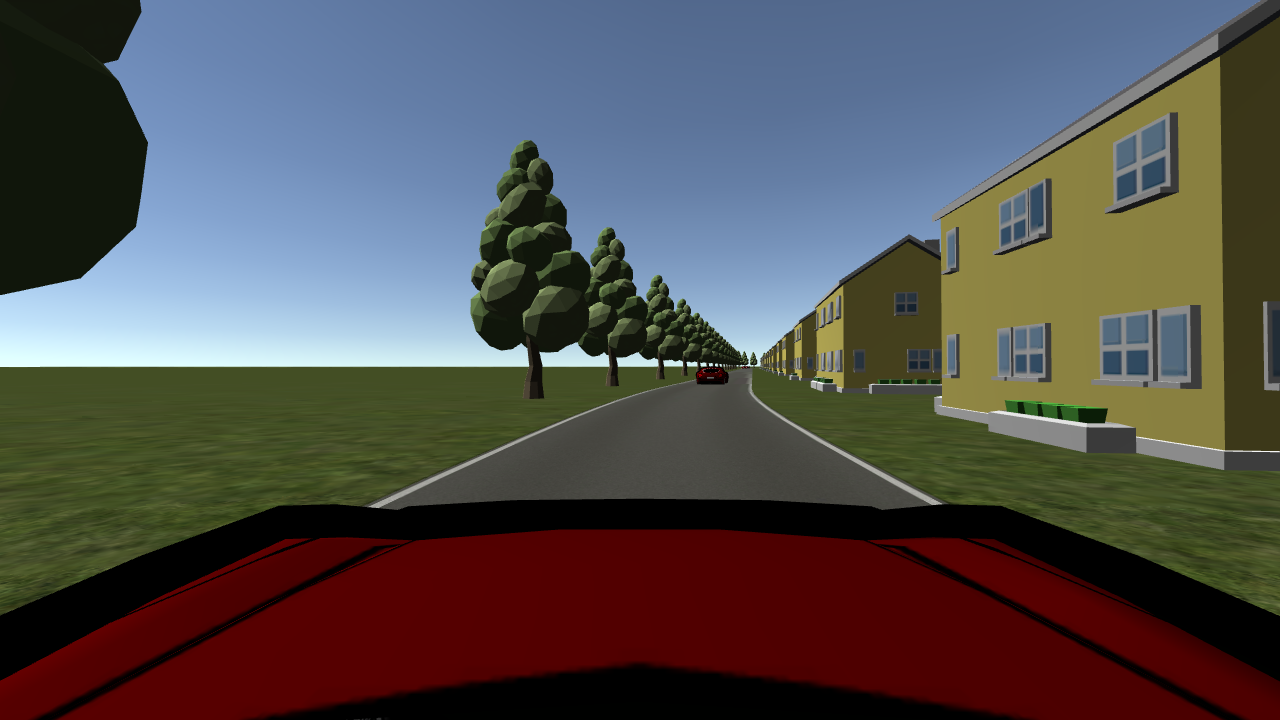
\includegraphics[width=\textwidth]{images/Chapter3/lane1.jpg}
%     \caption{Max. Lane = 1}
% 	\end{subfigure}
  
%   \begin{subfigure}[b]{0.8\linewidth}
% 		\centering
%     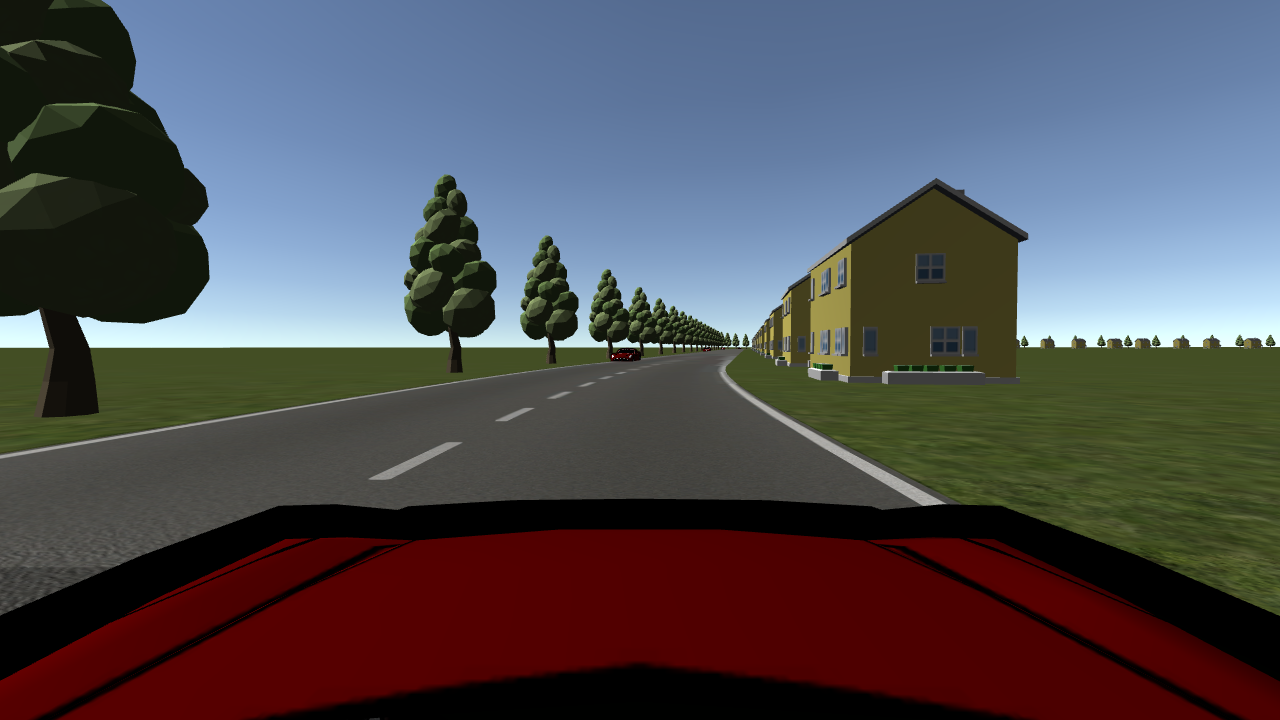
\includegraphics[width=\textwidth]{images/Chapter3/lane2.jpg}
%     \caption{Max. Lane = 2}
% 	\end{subfigure}\hfill
% 	\caption{Gathered images of Traffic scenes}
%   \label{}
% \end{figure}
